\subsubsection{Marginalizations}

When modeling a system, we sometimes want to ``hide'' details of a subsystem. The following operation
on SCMs that we call ``marginalization'' is a causal analogue of the marginalization of probability distributions.
The computer program analogy of the marginalization operation is to hide details within a subroutine.
Intuitively, a marginalization of an SCM over a subset of endogenous variables $L$ is obtained by first 
solving a subsystem (the structural equations
corresponding to the endogenous variables in $L$) followed by substituting the solution function of the 
subsystem into the remaining structural equations
(corresponding to the endogenous variables in $V\setminus L$).
\begin{Def}
  Let $\C{M} = \langle \Sin, \Send, \Srnd, \CX, P, f \rangle$ be an SCM and $L \subseteq \Send$ such that
  $\C{M}_{\doit(V\setminus L)}$ is uniquely solvable.
  Write $M = V \setminus L$ and let $\tilde{g}_L : \CX_{\Sin \cup M} \times \CXW \to \CX_L$
  be the unique solution function for $\C{M}_{\doit(M)}$.
  Then we call $\C{M}_{\setminus L} = \langle \Sin, M, \Srnd, \CX_{\Sin} \times \CX_{M} \times \CX_{\Srnd}, P, \tilde{f} \rangle$ with
  $$\tilde{f}(\xJ,x_{M},\xW) = f_{M}(\xJ,x_{M},\tilde{g}_L(\xJ,x_{M},\xW),\xW)$$
  the \emph{marginalization of $\C{M}$ over $L$}.
\end{Def}
For simple SCMs, marginalizations are obviously defined over any subset $L \subseteq \Send$.
%Note that all marginalizations of $\C{M}$ are equivalent, i.e., the marginalized causal mechanism is essentially unique.

Marginalization preserves unique solvability, as the following lemma shows.
\begin{Lem}\label{lem:marginalization_preserves_unique_solvability}
  Let $\C{M} = \langle \Sin, \Send, \Srnd, \CX, P, f \rangle$ be an SCM and $L \subseteq \Send$ such that
  $\C{M}_{\doit(V \setminus L)}$ is uniquely solvable.
  If $\C{M}$ is uniquely solvable then its marginalization $\C{M}_{\setminus L}$ is uniquely solvable, and the unique solution function for
  $\C{M}_{\setminus L}$ is just $g_M = \pr_M \circ g$, where $g : \CX_J \times \CX_W \to \CX_V$ is the 
  unique solution function for $\C{M}$, $M = V \setminus L$ and $\pr_M : \CXV \to \CX_M : x \mapsto x_M$ is the canonical projection on $M$.
\end{Lem}
\begin{proof}
  Let $\tilde{g}_L : \CX_{\Sin \cup M} \times \CXW \to \CX_L$
  be the unique solution function for $\C{M}_{\doit(M)}$.
  From the properties of the solution functions, we derive that
%  $\C{M}$ is uniquely solvable means there exists a measurable function $g : \CX_{J \cup W} \to \CX_V$ such  that
  for all $x \in \CX$,
  \begin{equation*}\begin{split}
  & \begin{cases}
    x_L = g_L(x_J,x_W) \\
    x_M = g_M(x_J,x_W) \\
  \end{cases}
  \iff x_V = g(x_J,x_W) \iff x_V = f(x) 
  \iff \begin{cases}
    x_L = f_L(x) \\
    x_M = f_M(x) \\
  \end{cases} \\
  & \iff \begin{cases}
    x_L = \tilde{g}_L(x_J,x_M,x_W) \\
    x_M = f_M(x_J,x_M,x_L,x_W) \\
  \end{cases}
  \iff \begin{cases}
    x_L = \tilde{g}_L(x_J,x_M,x_W) \\
    x_M = f_M(x_J,x_M,\tilde{g}_L(x_J,x_M,x_W),x_W) \\
  \end{cases} \\
  & \iff \begin{cases}
    x_L = \tilde{g}_L(x_J,x_M,x_W) \\
    x_M = \tilde{f}(x_J,x_M,x_W) \\
  \end{cases}
  \end{split}\end{equation*}
Hence for all $x_J \in \CX_J, x_W \in \CX_W, x_M \in \CX_M$:
$$x_M = g_M(x_J,x_W) \iff x_M = \tilde{f}(x_J,x_M,x_W).$$
Therefore, $g_M = \pr_M \circ g$ is the unique solution function for $\C{M}_{\setminus L}$, and the marginalized SCM $\C{M}_{\setminus L}$ is uniquely solvable.
\end{proof}
\begin{Rem}
This also directly implies that if $\C{M}$ is uniquely solvable and its marginalization $\C{M}_{\setminus L}$ over $L \subseteq V$ is defined, the observational Markov kernel of the marginalization is obtained by marginalizing the original observational Markov kernel:
$$P_{\C{M}_{\setminus L}}(X_{V\setminus L},X_W \mid \doit(X_J)) = P_{\C{M}}(X_{V\setminus L},X_W \mid \doit(X_J)).$$
\end{Rem}

Under certain conditions, hard interventions and marginalization commute (i.e., it does not matter in which
order we apply them).
\begin{Prp}\label{prp:interventions_marginalizations_commute}
Let $\C{M} = \langle \Sin, \Send, \Srnd, \CX, P, f \rangle$ be an SCM.
    For $L \subseteq V$ such that $\C{M}_{\doit(V\setminus L)}$ is uniquely solvable,
    and a hard intervention $\doit(T\dots)$ with target $T \subseteq \Sin \cup \Srnd \cup \Send$ (of any of the three variants) such that $L \cap T = \emptyset$:
    $$(\C{M}_{\doit(T\dots)})_{\setminus L} = (\C{M}_{\setminus L})_{\doit(T\dots)}.$$
\end{Prp}
\begin{proof}
  This follows by writing out the definitions and checking commutativity of
  the operations performed on the various components of the SCM tuple one-by-one. 
\end{proof}
Marginalization is also compatible with the twinning operation.
\begin{Prp}\label{prp:twinning_marginalization_commute}
Let $\C{M} = \langle \Sin, \Send, \Srnd, \CX, P, f \rangle$ be an SCM.
For $L \subseteq V$ such that $\C{M}_{\doit(V\setminus L)}$ is uniquely solvable,
$$(\C{M}_{\setminus L})^\twin = (\C{M}^\twin)_{\setminus (L\cup L')}.$$
\end{Prp}
\begin{proof}
  This follows by writing out the definitions and checking commutativity of
  the operations performed on the various components of the SCM tuple one-by-one.
\end{proof}

We will show that for simple SCMs, the marginalization operation preserves the causal semantics on the remaining variables. 
A key step is the following proposition, which gives conditions under which it does not matter whether we marginalize at once or in steps.
\begin{Prp}\label{prp:marginalization_commutes}
  Let $\C{M} = \langle \Sin, \Send, \Srnd, \CX, P, f \rangle$ be an SCM and $L_1, L_2 \subseteq \Send$ such that $L_1 \cap L_2 = \emptyset$.
  If $\C{M}_{\doit(V\setminus L_1)}$ is uniquely solvable, and
  $(\C{M}_{\setminus L_1})_{\doit((V\setminus L_1)\setminus L_2)}$ is uniquely solvable, then $\C{M}_{\doit(V\setminus(L_1\cup L_2))}$ is uniquely solvable, and in that case it does not matter if we first marginalize over $L_1$ and then $L_2$, or both at once, i.e:
  $$(\C{M}_{\setminus L_1})_{\setminus L_2} = \C{M}_{\setminus (L_1\cup L_2)}.$$
\end{Prp}
\begin{proof}
  Write $M_1 = V \setminus L_1$.
  Let $\tilde{g} : \CX_{J\cup M_1} \times \CXW \to \CX_{L_1}$ be the unique solution function of $\C{M}_{\doit(M_1)}$,
  i.e., for all $x \in \CX$:
  $$x_{L_1} = \tilde{g}(x_J,x_{M_1},x_W) \iff x_{L_1} = f_{L_1}(x).$$
  Let $\tilde{f} : \CX_J \times \CX_{M_1} \times \CXW \to \CX_{M_1}$ with
  $$\tilde{f}(x_J,x_{M_1},x_W) = f_{M_1}(x_J,x_{M_1},\tilde{g}(x_J,x_{M_1},x_W),x_W)$$
  be the causal mechanism of the marginal SCM $\C{M}_{\setminus L_1}$.

  If $(\C{M}_{\setminus L_1})_{\doit(V\setminus(L_1\cup L_2))}$ is uniquely solvable, it has a unique solution function
  $\dbtilde{g} : \CXJ \times \CX_{V\setminus (L_1\cup L_2)} \times \CXW \to \CX_{L_2}$, i.e., for all $x \in \CX$:
  $$x_{L_2} = \dbtilde{g}(x_J,x_{V\setminus(L_1\cup L_2)},x_W) \iff x_{L_2} = \tilde{f}_{L_2}(x_J,x_{L_2},x_{M_1\setminus L_2},x_W)$$
  Define the function $h : \CXJ \times \CX_{V\setminus(L_1\cup L_2)} \times \CXW \to \CX_{L_1 \cup L_2}$ by
  \begin{align*}
    h_{L_1}(x_J,x_{V\setminus(L_1\cup L_2)},x_W) &= \tilde{g}(x_J,x_{M_1\setminus L_2},\dbtilde{g}(x_J,x_{V\setminus(L_1 \cup L_2)},x_W),x_W) \\
    h_{L_2}(x_J,x_{V\setminus(L_1\cup L_2)},x_W) &= \dbtilde{g}(x_J,x_{V\setminus(L_1 \cup L_2)},x_W)
  \end{align*}
  Then for all $x \in \CX$:
  \begin{equation*}\begin{split}
%    & x_{L_1\cup L_2} = f_{L_1 \cup L_2}(x) \\
%    \iff &
    & \begin{cases}
      x_{L_1} &= f_{L_1}(x) \\
      x_{L_2} &= f_{L_2}(x) 
    \end{cases} \\
    \iff &
    \begin{cases}
      x_{L_1} &= \tilde{g}(x_J,x_{M_1},x_W) \\
      x_{L_2} &= f_{L_2}(x_J,x_{M_1},x_{L_1},x_W) 
    \end{cases} \\
    \iff &
    \begin{cases}
      x_{L_1} &= \tilde{g}(x_J,x_{M_1},x_W) \\
      x_{L_2} &= f_{L_2}(x_J,x_{M_1},\tilde{g}(x_J,x_{M_1},x_W),x_W) 
    \end{cases} \\
    \iff &
    \begin{cases}
      x_{L_1} &= \tilde{g}(x_J,x_{M_1\setminus L_2},x_{L_2},x_W) \\
      x_{L_2} &= \dbtilde{g}(x_J,x_{V\setminus(L_1 \cup L_2)},x_W)
    \end{cases} \\
    \iff &
    \begin{cases}
      x_{L_1} &= \tilde{g}(x_J,x_{M_1\setminus L_2},\dbtilde{g}(x_J,x_{V\setminus(L_1 \cup L_2)},x_W),x_W) \\
      x_{L_2} &= \dbtilde{g}(x_J,x_{V\setminus(L_1 \cup L_2)},x_W)
    \end{cases} \\
    \iff &
      x_{L_1\cup L_2} = h(x_J,x_{V\setminus(L_1\cup L_2)},x_W) 
  \end{split}\end{equation*}
  where in the first equivalence we used the unique solvability of $\C{M}_{\doit(M_1)}$, in the second
  equivalence we used substitution, in the third equivalence we used the unique solvability of
  $(\C{M}_{\setminus L_1})_{\doit(V\setminus (L_1\cup L_2))}$, in the fourth equivalence we used
  substitution again, and in the fifth equivalence we used the definition of $h$.
  Therefore, $h$ is the unique solution function for $\C{M}_{\doit(V\setminus(L_1\cup L_2)}$, which must therefore
  be uniquely solvable. By checking the definition, one concludes that $(\C{M}_{\setminus L_1})_{\setminus L_2} = \C{M}_{\setminus(L_1 \cup L_2)}$.
\end{proof}
\begin{Prp}\label{prp:marginalization_preserves_simplicity}
  Let $\C{M} = \langle \Sin, \Send, \Srnd, \CX, P, f \rangle$ be a simple SCM. For any $L \subseteq \Send$, 
  its marginalization $\C{M}_{\setminus L}$ is also simple.
\end{Prp}
\begin{proof}
  Let $T \subseteq J \cup W \cup V \setminus L$. 
  By Proposition~\ref{prp:interventions_marginalizations_commute}, 
  the marginalization commutes with the hard intervention:
  $$(\C{M}_{\setminus L})_{\doit(T)} = (\C{M}_{\doit(T)})_{\setminus L}.$$
  Because $\C{M}$ is simple, also $\C{M}_{\doit(T)}$ is simple (by Proposition~\ref{prp:hard_interventions_commute}), 
  and in particular it is
  uniquely solvable. From Lemma~\ref{lem:marginalization_preserves_unique_solvability} it follows that also
  its marginalization $(\C{M}_{\doit(T)})_{\setminus L}$ is uniquely solvable. 
  This means that $(\C{M}_{\setminus L})_{\doit(T)}$ is uniquely solvable. Since this
  holds for any $T \subseteq J \cup W \cup V \setminus L$, $\C{M}_{\setminus L}$ is simple.
\end{proof}
\begin{Cor}
  Let $\C{M} = \langle \Sin, \Send, \Srnd, \CX, P, f \rangle$ be a simple SCM.
  For $L_1, L_2 \subseteq \Send$ with $L_1 \cap L_2 = \emptyset$,
    $$(\C{M}_{\setminus L_1})_{\setminus L_2} = (\C{M}_{\setminus L_2})_{\setminus L_1} = \C{M}_{\setminus (L_1 \cup L_2)}.$$
\end{Cor}

These commutation relations and compatibilities now allow us to give a straightforward proof that
the causal semantics are preserved under marginalization.
While this holds generally \cite{BFPM21}, we will here only prove this for simple SCMs.
\begin{Thm}\label{Thm:various_equiv_marginalization}
  Let $\C{M} = \langle \Sin, \Send, \Srnd, \CX, P, f \rangle$ be a simple SCM, $L \subseteq \Send$, and
  $\C{M}_{\setminus L}$ its marginalization over $L$. Then $\C{M}$ and $\C{M}_{\setminus L}$ are observationally,
  interventionally and counterfactually equivalent w.r.t.\ $(V \cup W) \setminus L$.
\end{Thm}
\begin{proof}
  %The statement that $\C{M}$ and $\C{M}_O$ are observationally equivalent w.r.t.\ $O$ is Lemma~\ref{lem:obs_equiv_marginalization}.
  Write $M = V \setminus L$.
  We first show that the marginal Markov kernels $P_{\C{M}}(X_M,X_W \mid \doit(X_J))$ and $P_{\C{M}_{\setminus L}}(X_M,X_W \mid \doit(X_J))$ are the same.
%  By Theorem~\ref{thm:scm_unique_solvability}, the observational Markov kernels $P_{\C{M}}(X_V, X_W \mid X_J)$ and $P_{\C{M}_M}(X_M, X_W \mid X_J)$ exist and are unique. Hence, the marginal observational Markov kernels $P_{\C{M}}(X_M,X_W \mid X_J)$ and $P_{\C{M}_M}(X_M,X_W \mid X_J)$ exist and are unique. 
  The former is obtained as:
  $$P_{\C{M}}(X_M,X_W \mid \doit(X_J)) = (\pr_{M\cup W} \circ (g,\id_{\CXW}))_*(P) = (g_{M},\id_{\CXW})_*(P),$$
  where $g : \CXJ \times \CXW \to \CXV$ is the unique solution function of $\C{M}$ and
  $\pr_{M\cup W} : \CX_{V \cup W} \to \CX_{M\cup W}$ is the canonical projection on the $M\cup W$ components. 
  The latter is obtained as:
  $$P_{\C{M}_{\setminus L}}(X_M,X_W \mid \doit(X_J)) = (g_M,\id_{\CXW})_*(P)$$
  since by Lemma~\ref{lem:marginalization_preserves_unique_solvability}, $g_M$ is the (unique) solution function of $\C{M}_{\setminus L}$.
  This means that both push-forwards are identical.

  Let $T \subseteq M \cup W$. Then $(\C{M}_{\setminus L})_{\doit(T)} = (\C{M}_{\doit(T)})_{\setminus L}$ by
  Proposition~\ref{prp:interventions_marginalizations_commute}. 
  The observational equivalence of $\C{M}_{\doit(T)}$ and $(\C{M}_{\doit(T)})_{\setminus L}$ w.r.t.\ $(M \cup W) \setminus T$ hence implies the observational equivalence of $\C{M}_{\doit(T)}$ and $(\C{M}_{\setminus L})_{\doit(T)}$ w.r.t.\ $(M \cup W) \setminus T$. 
  Since this holds for all $T \subseteq M \cup W$, $\C{M}$ and $\C{M}_{\setminus L}$ are interventionally equivalent w.r.t.\ $M \cup W$.

  Finally, $(\C{M}_{\setminus L})^\twin = (\C{M}^\twin)_{\setminus (L \cup L')}$ by Proposition~\ref{prp:twinning_marginalization_commute}. Since $\C{M}^\twin$ and its marginalization
  $(\C{M}^\twin)_{\setminus (L \cup L')}$ are interventionally equivalent w.r.t.\ $M \cup M' \cup W$, 
  $\C{M}$ and $\C{M}_{\setminus L}$ are counterfactually equivalent w.r.t.\ $M \cup W$.
\end{proof}
So the marginalization operation indeed effectively hides the details of a subsystem, while preserving all causal semantics on the remaining part.

\subsubsection{Graphs of SCMs}

A useful abstraction of an SCM is its graph. 
The directed edges in the graph of an SCM will express the following ``parent''-relation that captures \emph{functional dependencies} in the structural equations / causal mechanisms.
\begin{Def}\label{def:scm_parent}
  Let $\C{M} = \langle \Sin, \Send, \Srnd, \CX, P, f \rangle$ be an SCM.
  For $i \in \Sin \cup \Send \cup \Srnd$ and $j \in \Send$, we say that
  \emph{$i$ is a parent of $j$ according to $\C{M}$} if there does not exist a measurable function 
  $\tilde f_j : \CX_{(\Sin\cup\Send\cup\Srnd) \setminus \{i\}} \to \CX_j$
  such that for all $x \in \CX$,
  $$x_j = f_j(x) \iff x_j = \tilde f_j(x_{\setminus i}),$$
  where $x_{\setminus i}$ is shorthand for $x_{(\Sin\cup\Send\cup\Srnd)\setminus\{i\}}$.
\end{Def}
In words, $i$ is parent of $j$ if the causal mechanism for $j$ is equivalent to one that is constant with respect to its input component $i$.
By definition, exogenous (input and random) variables have no parents.
Note that the parent-relationship is preserved under equivalence.
Using directed edges to encode the parent-relationship, we define the graph of the SCM.
\begin{Def}\label{def:scm_graph}
  Let $\C{M} = \langle \Sin, \Send, \Srnd, \CX, P, f \rangle$ be an SCM.
  The CDG $\langle \Sin, \Send \cup \Srnd, E \rangle$ with
  input nodes $\Sin$, output nodes $\Send\cup\Srnd$, and
  directed edges 
  $$E = \{i \to j : i \in \Sin\cup\Srnd\cup\Send, j\in\Send: \text{$i$ is parent of $j$ according to $\C{M}$}\}$$
  is called the \emph{graph of the SCM} and will be denoted as $G(\C{M})$.
\end{Def}
Since the parent-relationship is preserved under equivalence, equivalent SCMs have the same graphs.
However, observationally equivalent SCMs may have different graphs, and even interventionally equivalent
SCMs may have different graphs.
%\begin{Exc}
%  Do graphs of counterfactually equivalent SCMs have the same directed edges between endogenous variables?
%  Give a proof or a counterexample.
%\end{Exc}

\begin{Eg}
  The SCM in Example~\ref{eg:equivalent_scm}, 
  with endogenous variable $X$ and exogenous random variable $W$ and structural equation
  $$X = -X^3 + X + W$$
  has graph:\\
  \centerline{\begin{tikzpicture}
    \node[var] (W) at (0,0) {$W$};
    \node[var] (X) at (1.5,0) {$X$};
    \draw[arr] (W) -- (X);
  \end{tikzpicture}}
  It does not have a self-cycle at $X$, since $X$ is not a parent to itself: 
  the structural equation is equivalent to $$X = \sqrt[3]{W},$$
  where $X$ does not appear on the r.h.s..
  
  On the other hand, the graph of the SCM in Example~\ref{eg:self_cycle} 
  with structural equation 
  $$X = W X + c$$
  does have a self-cycle at $X$:\\
  \centerline{\begin{tikzpicture}
    \node[var] (W) at (0,0) {$W$};
    \node[var] (X) at (1.5,0) {$X$};
    \draw[arr] (W) -- (X);
    \draw[arr,in=30,out=-30,looseness=5] (X) edge (X);
  \end{tikzpicture}}
\end{Eg}
Self-cycles are a warning sign of complications with respect to solvability.
They are of no concern when restricting to the class of simple SCMs.
\begin{Prp}
  For $j \in V$, we have that there is a self-cycle $j \to j$ in $G(\C{M})$ if and only if
  $\C{M}_{\doit(V\setminus \{j\})}$ is \emph{not} uniquely solvable. 
  In particular, graphs of simple SCMs have no self-cycles.
\end{Prp}

While the graph explicitly represents all exogenous random variables, coarser
representations obtained via (graphical) marginalization are also useful.
\begin{Rem}
  An often used convention is to consider \emph{all} exogenous random variables to be latent. 
  In that case, a useful graph
  to consider is the marginalization $(G)^{\setminus \Srnd}(\C{M})$ of the graph $G(\C{M})$. 
  The marginal CDMG $G^{\setminus \Srnd}(\C{M}) = \langle \Sin, \Send, E, L \rangle$ has
  input nodes $\Sin$, output nodes $\Send$, directed edges
  $$E = \{i \to j : i \in \Sin\cup\Send, j\in\Send: \text{$i$ is parent of $j$ according to $\C{M}$}\}$$
  and bidirected edges
  $$L = \{j \oto k : j \in \Send, k \in \Send, j \ne k: \text{$j$ and $k$ have a common parent $i\in\Srnd$ according to $\C{M}$}\}.$$
  In other words, $G^{\setminus \Srnd}(\C{M})$ is obtained from $G(\C{M})$ by replacing the nodes representing the exogenous random
  variables and their outgoing directed edges with bidirected edges, i.e.,
  any pattern $\ot i \to$ with $i \in \Srnd$ is replaced by $\oto$.
\end{Rem}

We already provided definitions for hard interventions on graphs (Definition~\ref{def:G_hard_intervention})
and for marginalizations (latent projections) of graphs (Definition~\ref{def:G_marginalization}). 
We can also define a twinning operation on graphs. We will only define this for graphs without bidirected edges.
\begin{Def}\label{def:G_twinning}
  Let $G=\langle J,V \cup W,E\rangle$ be a CDG such that $\Pa^G(W) = \emptyset$. Write $J' := \{j' : j \in J\}$
  and $V' := \{v' : v \in V\}$ for copies of $J$ and $V$, respectively.
  The \emph{twinned graph
  $G^{\twin(J,V)}$} is defined as the CDG $\langle J \dot\cup J', V \dot\cup V' \cup W, \tilde{E}\rangle$ with directed edges
  $$\tilde{E} := E \cup \{w \to v' : w \in W, v \in V, w \to v \in E\} \cup \{i' \to v' : i \in J \cup V, v \in V, i \to v \in E\}.$$
  In words, we copy the nodes $J \cup V$ (but not the nodes $W$) and copy the edges accordingly.
\end{Def}

The mapping that maps an SCM to its graph is compatible with the elementary operations on SCMs.
\begin{Prp}\label{prp:compatibility_graph}
  Let $\C{M} = \langle \Sin, \Send, \Srnd, \CX, P, f \rangle$ be an SCM. Then
  \begin{itemize}
    \item Hard interventions: for $T \subseteq J \cup V \cup W$, 
      $$G(\C{M}_{\doit(T)}) = G(\C{M})_{\doit(T)}.$$
    \item Twinning:
      $$G(\C{M})^{\twin(J\cup V)} = G(\C{M}^\twin).$$
    \item Marginalizations: If $\C{M}$ is simple, then for $L \subseteq V$, 
      $$G(\C{M}_{\setminus L}) \subseteq G(\C{M})^{\setminus L}.$$
  \end{itemize}
\end{Prp}
\begin{proof}
  The first two statements follow by writing out the definitions. The third one is somewhat more involved. We will
  first prove it in case $L = \{\ell\}$ consists of a single node. 
  Let $G = G(\C{M})$.
  By using the definition of the parent relation (repeatedly), we can find a function $\tilde{f}_\ell : \CX_{\Pa^G(\ell)} \to \CX_\ell$ such that
  for all $x \in \CX$:
  $$x_\ell = f_\ell(x) \iff x_\ell = \tilde{f}_\ell(x_{\Pa^G(\ell)}).$$
  Since $\ell \notin \Pa^G(\ell)$ because $\C{M}$ is simple, %(more generally: because $\C{M}_{\doit(V\setminus\{\ell\})}$ is uniquely solvable),
  the unique solution function
  $\tilde{g}_\ell : \CX_{J \cup V \setminus \{\ell\} \cup W} \to \CX_\ell$ of $\C{M}_{\doit(V\setminus \{\ell\})}$
  satisfies $\tilde{g}_\ell(x_{\setminus \ell}) = \tilde{f}_\ell(x_{\Pa^G(\ell)})$, i.e., it only depends on the parents of $\ell$.
  When constructing the marginalized causal mechanism for $\C{M}_{\setminus \{\ell\}}$, we substitute 
  $\tilde{g}_\ell(x_{\setminus \ell})$ into the $\ell$'th input of the causal mechanism $f_j$ of $\C{M}$, for $j \in V\setminus \{\ell\}$.
  Since $\tilde{g}_\ell$ only depends on $\Pa^G(\ell)$,
  we get that $\Pa^{\tilde G}(j) \subseteq \Pa^G(j) \setminus \{\ell\} \cup \Pa^G(\ell)$, where $\tilde{G} = G(\C{M}_{\setminus \ell})$.
  But we also have $\Pa^{G^{\setminus \{\ell\}}}(j) = \Pa^G(j) \setminus \{\ell\} \cup \Pa^G(\ell)$ by definition of the graphical marginalization. 
  Hence $\Pa^{\tilde G}(j) \subseteq \Pa^{G^{\setminus \{\ell\}}}$ for all $j \in V\setminus \{\ell\}$, and we have shown that $G(\C{M}_{\setminus \{\ell\}}) \subseteq G(\C{M})^{\setminus \{\ell\}}$.
  For the general case, we can make use of induction and the facts that both for
  graphs and simple SCMs, we can obtain a marginalization over a subset by repeatedly marginalizing out a single remaining node in the subset, in arbitrary order.
\end{proof}

A subclass of SCMs that is often considered are acyclic SCMs.
\begin{Def}
  An SCM $\C{M}$ is called \emph{acyclic} if its graph $G(\C{M})$ is acyclic.
\end{Def}
If one models static systems, then using acyclic SCMs
rules out the presence of causal cycles (e.g., feedback loops) in the system.
Acyclic SCMs are a subclass of the more general class of simple SCMs.
\begin{Prp}
  Acyclic SCMs are simple.
\end{Prp}
\begin{proof}
  We first show that acyclic SCMs are uniquely solvable. Let $\C{M}$ be an acyclic SCM. Its
  graph $G := G(\C{M})$ is acyclic, and hence has a topological order $<$. Consider $f_v$, the
  causal mechanism for $v \in V$. The parents $\Pa^G(v)$ precede $v$ in the topological order.
  Since $f_v$ can be rewritten to be constant in the non-parents of $v$ (similar to how this
  was done in the proof of Proposition~\ref{prp:compatibility_graph}), 
  we can consider $f_v : \CX \to \CX_v$ as a function
  $f_v : \CX_{\Pred_<^{G}(v)} \to \CX_v$ instead. We can then inductively define the components
  $$g_v : \CXJ \times \CXW \to \CX_v : 
    (\xJ,\xW) \mapsto f_v(g_{\Pred_<^{G}(v)}(\xJ,\xW))$$
  that together form a solution function $g : \CX_{J\cup W} \to \XV$.
  This construction also exhibits the uniqueness of $g : \CX_{J\cup W} \to \XV$.

  Next consider $\C{M}_{\doit(T)}$, the intervened SCM for a hard intervention on $\C{M}$ with target $T \subseteq V \cup W \cup J$. 
  It has graph $G(\C{M}_{\doit(T)}) = G_{\doit(T)}$, whose edges form a subset of the edges of $G$ (but
  where some output nodes have become input nodes), and hence is also acyclic. 
  Therefore, also $\C{M}_{\doit(T)}$ is uniquely solvable. Since this holds for all targets $T \subseteq V \cup W \cup J$,
  we conclude that $\C{M}$ is simple.
\end{proof}

\begin{figure}\centering
  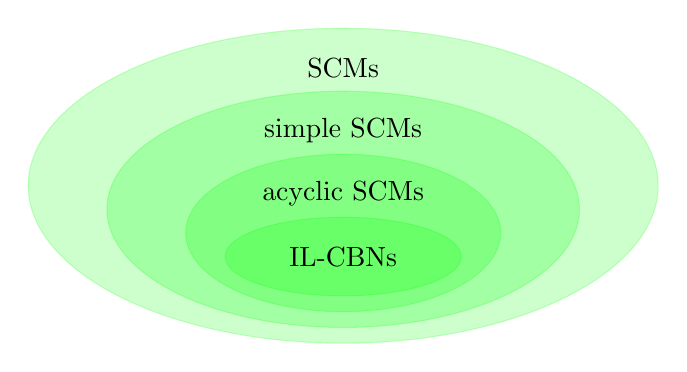
\begin{tikzpicture}
      \begin{scope}
        \draw[draw=green,fill=green,opacity=0.2] (0,0) ellipse (1.5cm and 0.5cm);
        \draw[draw=green,fill=green,opacity=0.2] (0,0.3) ellipse (2cm and 1cm);
        \draw[draw=green,fill=green,opacity=0.2] (0,0.6) ellipse (3cm and 1.5cm);
        \draw[draw=green,fill=green,opacity=0.2] (0,0.9) ellipse (4cm and 2cm);
        \node at (0,0) {IL-CBNs};
        \node at (0,0.8) {acyclic SCMs};
        \node at (0,1.6) {simple SCMs};
        \node at (0,2.4) {SCMs};
      \end{scope}
  \end{tikzpicture}
  \caption{Venn diagram for different causal modeling classes.\label{fig:venn_diagram_scms}}
\end{figure}
Figure~\ref{fig:venn_diagram_scms} shows a Venn diagram to illustrate how the different
classes of causal models that we introduced are related.
Acyclic SCMs are more expressive than IL-CBNs, because they also model counterfactuals.
Simple SCMs are more expressive than acyclic SCMs because they can model (sufficiently
weak) causal cycles. SCMs in general are even more expressive because they can also
model stronger cycles that not necessarily lead to unique solvability under any hard
intervention, but this generality comes with a substantially increased complexity of
the theory and interpretability. Simple SCMs form a ``sweet spot'' in the sense that they allow cyclic
relationships yet their theory is not much more complicated than that of acyclic SCMs:
the main difference consists in replacing $d$-separation with $\sigma$-separation.

\subsubsection{(Alternative definition of $\sigma$-blocking)}

Revisit Definition~\ref{def:sigma_blocking} of $\sigma$-blocking. In the literature, one also encounters
a slightly different notion with the same name. In this optional section, we will clarify the relationship
between the two. For the rest of the course, we will keep using Definition~\ref{def:sigma_blocking}.
\begin{Def}\label{def:sigma_blocking_2}
  Let $G=\langle J,V,E,L \rangle$ be a CDMG, $C \ins J \cup V$ a subset of nodes and $\pi$ a walk (or path) in $G$:
  \[ \pi =\lp  v_0 \sts \cdots \sts v_n \rp.  \]
\begin{enumerate}
  \item
    We say that the walk (or path) $\pi$ is \emph{$C$-$\sigma'$-blocked} or \emph{$\sigma'$-blocked by $C$} if either:
      \begin{enumerate}[label=\roman*.)]
          \item $v_0 \in C$ or $v_n \in C$ or:
          \item there are two adjacent edges in $\pi$ of one of the following forms:
              \[\begin{array}{rccl}
  \text{ left chain: } & v_{k-1} \ot v_k \ots v_{k+1} & \text{ with } & v_k \in C \land v_k \notin \Sc^G(v_{k-1}),\\
  \text{ right chain: } & v_{k-1} \sto v_k \to v_{k+1} & \text{ with } & v_k \in C \land v_k \notin \Sc^G(v_{k+1}),\\
  \text{ fork: } & v_{k-1} \ot v_k \to v_{k+1} & \text{ with } & v_k \in C \land v_k \notin \Sc^G(v_{k-1}) \cap \Sc^G(v_{k+1}),\\
                \text{ collider: } & v_{k-1} \sto v_k \ots v_{k+1} & \text{ with } & v_k \notin \Anc^G(C).
              \end{array}\]
      \end{enumerate}
  \item We say that the walk (or path) $\pi$ is \emph{$C$-$\sigma'$-open} if it is not $C$-$\sigma'$-blocked. 
\end{enumerate}
\end{Def}
The only difference is in the condition for a collider node $v_k$: to $\sigma$-block
a walk one needs $v_k \not\in C$, whereas to $\sigma'$-block a walk one needs $v_k \not\in \Anc^G(C)$.

The following lemma will be convenient to relate the notions.
\begin{Lem}\label{lem:replace_walk}
Let $G = \langle V, J, E, L \rangle$ be a CDMG, $C \subseteq V \cup J$ and $\pi = (v_0,\dots,v_n)$ be a $C$-$\sigma'$-open walk in $G$. 
Suppose $v_i \in \Sc^G(v_j)$ with $i < j$.
We can then replace the subwalk $v_i, \dots, v_j$ of $\pi$ by 
  \begin{enumerate}[label=(\roman*)]
    \item a shortest directed path $v_i \to \dots \to v_j$ in $G$ if $j = n$ or if $v_j \to v_{j+1}$ on $\pi$, or
    \item a shortest directed path $v_i \ot \dots \ot v_j$ in $G$ otherwise,
  \end{enumerate}
that is entirely within $\Sc^G(v_i)$ and such that the modified walk $\pi'$ is still $C$-$\sigma'$-open.
\end{Lem}
\begin{proof}
$\pi'$ cannot become $C$-$\sigma'$-blocked by one of the initial nodes $v_0 \dots v_{i-1}$ or one of the final nodes $v_{j+1} \dots v_n$ on $\pi'$, since these nodes occur in the same local configuration on $\pi$ and do not $C$-$\sigma'$-block $\pi$ by assumption.
Furthermore, $\pi'$ cannot become $C$-$\sigma'$-blocked through one of the nodes strictly between $v_i$ and $v_j$ on $\pi'$ (if there are any), since these nodes are all non-endpoint non-colliders that only point to nodes in the same strongly connected component on $\pi'$.
Because $\pi$ is $C$-$\sigma'$-open, $v_j \notin C$ if $j = n$ or if $v_j \to i_{j+1}$ on $\pi$. 
This holds in particular in case (i). 
Similarly, $v_i \notin C$ if $i = 0$ or $v_{i-1} \ot v_i$ on $\pi$.

In case (i), $\pi'$ is not $C$-$\sigma'$-blocked by $v_j$ because $v_j$ is a non-collider on $\pi'$ but $v_j \notin C$. 
Also $v_i$ does not $C$-$\sigma'$-block $\pi'$. Indeed, assume $v_i \ne v_j$ (otherwise there is nothing to prove).
If $i = 0$, or if $i > 0$ and $v_{i-1} \ot v_i$ on $\pi'$, then the same holds for $\pi$ and hence $v_i \notin C$; $v_i$ is then a non-collider on $\pi'$, but $v_i \notin C$. 
If $i > 0$ and $v_{i-1} \sto v_i$ on $\pi'$ then $v_i$ is a non-endpoint non-collider on $\pi'$ that does not point to a node in another strongly connected component.

Now consider case (ii). 
If $i = 0$ or $v_{i-1} \ot v_i$ on $\pi'$ then this case is analogous to case (i). 
So assume $i > 0$ and $v_{i-1} \sto v_i$ on $\pi'$. 
%If $v_i$ is an endpoint of $\pi'$, then $v_i = v_j$ and $k = n$ and therefore $v_j \notin C$, and hence $v_i$ and $v_j$ do not $C$-$\sigma'$-block $\pi'$. 
$v_i$ must be a collider on $\pi'$ (whether $v_i = v_j$ or not). 
Then on the subwalk of $\pi$ between $v_i$ and $v_j$ there must be a directed walk from $v_i$ to a collider that is in $\Anc^G(C)$, which implies that $v_i \in \Anc^G(C)$. Hence, $v_i$ will not $C$-$\sigma'$-block $\pi'$. 
Also $v_j$ cannot $C$-$\sigma'$-block $\pi'$.
Indeed, assume $v_i \ne v_j$ (otherwise there is nothing to prove). 
Since $v_j \ots v_{j+1}$ on $\pi'$, $v_j$ is a non-endpoint non-collider on $\pi'$ that does not point to a node in another strongly connected component.
\end{proof}
With the help of this lemma, we can prove that Definition~\ref{def:sigma_blocking_2} indeed serves as an alternative to 
Definition \ref{def:sigma_blocking}.
\begin{Prp}\label{prp:sigma_opens}
  Let $G = \langle J, V, E, L \rangle$ be a CDMG. For $C \subseteq J \cup V$, and $i, j \in J \cup V$, the following are
  equivalent:
  \begin{enumerate}
    \item there exists a $C$-$\sigma$-open walk between $i$ and $j$ in $G$;
    \item there exists a $C$-$\sigma'$-open walk between $i$ and $j$ in $G$;
    \item there exists a $C$-$\sigma'$-open path between $i$ and $j$ in $G$.
  \end{enumerate}
\end{Prp}
\begin{proof}
$1 \implies 2$: Suppose there exists a $C$-$\sigma$-open walk between $i$ and $j$.
%Then all non-colliders are either not in $C$, or only point towards nodes in the same strongly connected component;
%all colliders are in $C$. 
All colliders are in $C$, and hence in $\Anc^G(C)$. So this same walk is also $C$-$\sigma'$-open. 

$2 \implies 1$: Suppose there exists a $C$-$\sigma'$-open walk between $i$ and $j$. 
%Then all non-colliders are either not in $C$, or only point towards nodes in the same strongly connected component; 
Then all colliders are in $\Anc^G(C)$. If a collider is not in $C$, we can extend the walk by replacing this collider 
$\sto v \ots$ by the walk 
$\sto v \to \dots \to c \ot \dots \ot v \ots$ consisting of a directed walk starting from $v$ towards the first
node $c$ in $C$ it encounters, and from there tracing back the same walk in opposite direction to $v$. All nodes on this
walk except for $c$ ($v$ included) are non-colliders not in $C$. Extending this walk in such a way for each
collider not in $C$, we obtain an extended walk that is $C$-$\sigma$-open.

$2 \implies 3$:
%It suffices to show that if there exists a $C$-$\sigma$-open walk between $i$ and $j$ in $G$, there exists a $C$-$\sigma'$-open path between $i$ and $j$ in $G$. 
Let $\pi = (v_0,\dots,v_n)$ be a $C$-$\sigma'$-open walk between nodes $v_0$ and $v_0$ in $G$. 
If a node $w$ occurs more than once on $\pi$, let $v_i$ be the first node on $\pi$ and $v_j$ be the last node on $\pi$ that are in $\Sc^G(w)$.
We now use Lemma~\ref{lem:replace_walk} to construct a new walk $\pi'$ from $\pi$ by replacing the subwalk between $v_i$ and $v_j$ of $\pi$ by a particular directed path in $\Sc^G(w)$ between $v_i$ and $v_j$ in such a way that $\pi'$ is still $C$-$\sigma'$-open.
In $\pi'$, the number of nodes that occurs more than once is at least one less than in $\pi$, and all nodes within $\Sc^G(w)$ occur within a single segment.
This replacement procedure can be repeated until no nodes occur more than once. We have then obtained a
$C$-$\sigma'$-open path between $v_0$ and $v_n$.

$3 \implies 2$: trivial.
\end{proof}
Hence, it does not matter which of the two notions we use in the definition of $\sigma$-separation.
When checking $\sigma$-separation in a graph ``by hand'', we usually use the third formulation, since there are only a finite
number of paths to check. In proofs, though, it often is easier to make use of walks, since these can be concatenated into walks
(while one cannot in general concatenate two paths and again obtain a path).

\subsubsection{Acyclifications}

It is possible to reformulate the notion of $\sigma$-separation in terms of $d$-separation on a modified and acyclic graph
by making use of the following construction, which will be the main tool to extend the acyclic theory for
IL-CBNs to cyclic SCMs. The construction was first proposed in the context of CBNs by \cite{Spirtes94,Spirtes95}.
\begin{Def}\label{def:cdg_acyclification}
  Given a CDMG $G = \langle J, V, E, L \rangle$, we call a CADMG $G' = \langle J, V, E', L' \rangle$
  an \emph{acyclification of $G$} if
  \begin{enumerate}[label=(\roman*)]
    \item $G'$ is acyclic;
    \item $G'$ has the same input nodes $J$ and output nodes $V$ as $G$;
    \item for any pair of nodes $\{i,j\}$ such that $i \not\in\Sc^G(j)$:
      \begin{enumerate}
      \item $i \to j \in E'$ iff there exists a node $j' \in \Sc^G(j)$ such that $i \to j' \in E$;
      \item $i \oto j \in L'$ iff there exist nodes $i' \in \Sc^G(i), j' \in \Sc^G(j)$ such that $i' \oto j' \in L$;
      \end{enumerate}\label{def:acyclification_inter_scc}
    \item for any pair of distinct nodes $\{i,j\}$ such that $i \in\Sc^G(j)$: $i \to j \in \C{E}'$ or $i \ot j \in \C{E}'$ or $i \oto j \in \C{F}'$.\label{def:acyclification_intra_scc}
  \end{enumerate}
\end{Def}

\begin{comment}
Before we state and prove its main property, we start with a little lemma.
\begin{Lem}\label{lem:acyclification_ancestors}
Let $G$ be a CDMG and $G'$ an acyclification of $G$. 
For any node $j \in J \cup V$: if $i \in \Anc^G(j)$ then there
exists $i' \in \Sc^G(i)$ such that $i' \in \Anc^{G'}(j)$.
Vice versa: if $i \in \Anc^{G'}(j)$ then $i \in \Anc^G(j)$.
\end{Lem}
\begin{proof}
If there exists a directed walk from $i$ to $j$ in $G$,
this walk can be partitioned into maximal segments that are contained within a single strongly connected component of $G$ each.
By the definition of $G'$, there exists a directed walk in $G'$ that contains the right-most node only for each segment
(keeping the same ordering of the segments). 
Its end node will be $j$, but its start node may be a node $i' \in \Sc^G(i)$ that differs from $i$.

If there exists a directed walk from $i$ to $j$ in $G'$,
then we can replace each edge $u \to v$ on this walk (if it is not present in $G$) by a directed walk
$u \to v' \to \dots \to v$ where $v' \to \dots \to v$ is entirely within $\Sc^G(v)$, by definition of $G'$. 
In this way we obtain a directed walk in $G$ from $i$ to $j$.
\end{proof}
\end{comment}
The important property of acyclifications is that they can be used to express $\sigma$-separation in a (possibly cyclic) graph
in terms of $d$-separation in an acyclification.
\begin{Prp}\label{prp:sigma_sep_as_d_sep}
  Let $G = \langle J, V, E, L \rangle$ be a CDMG and $G' = \langle J, V, E', L' \rangle$ an acyclification of $G$. 
  Then for $A, B, C \subseteq V \cup J$ (not necessarily disjoint) subsets of nodes,
  $$A \Perp^\sigma_G B \given C \iff A \Perp^\sigma_{G'} B \given C \iff A \Perp^d_{G'} B \given C$$
\end{Prp}
\begin{comment}\begin{proof}
We will show that there is a $C$-$\sigma'$-open walk between $A$ and $B \cup J$ in $G$ if and only
if there is a $C$-$\sigma'$-open walk between $A$ and $B \cup J$ in $G'$. This is equivalent to the
existence of a $C$-$\sigma$-open walk between $A$ and $B \cup J$ in $G'$ by Proposition~\ref{prp:sigma_opens}. 
Since $G'$ is acyclic, this
is in turn equivalent to the existence of a $C$-$d$-open walk between $A$ and $B \cup J$ in $G'$.

$\implies$: Suppose there is a $C$-$\sigma'$-open walk $\pi = (v_0, \dots, v_n)$ between $A$ and $B \cup J$ in $G$. 
All its colliders are in $\Anc^G(C)$
and all its non-colliders are either not in $C$, or otherwise, point only to nodes in the same strongly connected component.
Note that each edge between two nodes in different strongly connected components in $G$ is also present in $G'$.
Edges between two nodes in the same strongly connected component, however, may not be present in $G'$.
Therefore, we will replace these edges with walks in $G'$. 
We may also need to replace colliders in $\Anc^G(C)$ with colliders in $\Anc^{G'}(C)$.
Consider a subwalk $(v_i,\dots,v_j)$ of maximum length that is entirely contained within a strongly connected component in $G$
(with possibly $i=j$).
We distinguish different cases and show for each case
how this subwalk can be replaced by a subwalk in $G'$.
\begin{enumerate}[label=(\roman*)]
  \item 
$\sto v_i \cdots v_j \ots$: the subwalk between $v_i$ and $v_j$ has to contain a collider, say $w$,
which must be in $\Anc^G(C)$ since the walk between $i$ and $j$ is $C$-$\sigma'$-open.
By Lemma~\ref{lem:acyclification_ancestors}, there must exist a node $w' \in \Sc^G(w)$
that is in $\Anc^{G'}(C)$. Thus we can replace this subwalk by
$\sto w' \ots$ in $G'$ such that $w'$ becomes a collider in $\Anc^{G'}(C)$.

\item
$(\ot) v_i \cdots v_j \ots$:\footnote{We put parentheses around the first directed edge to indicate that
this case also applies if $v_i$ is an endnode, i.e., if $i = 0$.} 
here $v_i$ is a non-collider pointing to another strongly-connected component or $v_i$ is an endnode,
and in both cases, $v_i \notin C$. Therefore, we can replace the subwalk by $(\ot) v_i \ots$ in $G'$,
such that $v_i$ becomes a non-collider not in $C$.

\item
$\sto v_i \cdots v_j (\to)$: analogous to the previous case, we can replace it by $\sto v_j (\to)$ in $G'$,
such that $v_j$ becomes a non-collider not in $C$.

\item
$(\ot) v_i \cdots v_j (\to)$: 
$v_i,v_j$ are both not in $C$ by assumption. If $i = j$, we replace this subwalk by $(\ot) v_i (\to)$ 
such that $v_i$ becomes a non-collider not in $C$. If $i < j$, we replace this subwalk by
$(\ot) v_i \sts v_j (\to)$ with $v_i \sts v_j$ any edge connecting $v_i$ and $v_j$ in $G'$,
such that both $v_i$ and $v_j$ become non-colliders not in $C$.
\end{enumerate}
By replacing all maximal subwalks of the original walk $\pi$ that are contained within a single strongly connected
component of $G$ in this way, we obtain a walk in the acyclification $G'$ that is $C$-$\sigma'$-open by construction.
Note that the modified walk has the same endpoints ($v_0$ and $v_n$) as the original walk.

$\impliedby$: Suppose there is a $C$-$\sigma'$-open walk $\pi$ between $A$ and $B \cup J$ in $G'$.
All its colliders are in $\Anc^{G'}(C)$ (and hence in $\Anc^G(C)$ by Lemma~\ref{lem:acyclification_ancestors}), and
all its non-colliders are not in $C$. 
We will construct a walk $\pi'$ in $G$ with the same endpoints as $\pi$ that is $C$-$\sigma'$-open.

First, we replace all non-trivial maximum subwalks $v_i \sts \dots \sts v_j$ on $\pi$ consisting entirely
of edges between nodes in the same strongly connected component in $G$ by
a directed path $v_i \to \dots \to v_j$ or $v_i \ot \dots \ot v_j$ 
entirely in $\Sc^G(i)$ in the same way as in Lemma~\ref{lem:replace_walk}.
By the same reasoning as in the proof of the lemma, both $v_i$ and $v_j$ will become
either colliders in $\Anc^G(C)$, or non-colliders not in $C$, or non-colliders in $C$
that only point to a node in the same strongly connected component of $G$.

Next, for any directed edge $i \to j$ on $\pi$ with $j \notin \Sc^G(i)$, there
must be a $j' \in \Sc^G(j)$ such that $i \to j'$ is present in $G$, and hence there must be a directed path
$j' \to \dots \to j$ entirely in $\Sc^G(j)$ such that we can use
$i \to j' \to \dots \to j$ as replacement in $G$ of the edge $i \to j$ on $\pi$.
Similarly, for any bidirected edge $i \oto j$ on $\pi$ with $j \notin \Sc^G(i)$, there
must be $i' \in \Sc^G(i)$ and $j' \in \Sc^G(j)$ such that $i' \oto j'$ is present in $G$, 
and hence there must be a walk $i \ot \dots \ot i' \oto j' \to \dots \to j$ in $G$, where
$i \ot \dots \ot i'$ is entirely in $\Sc^G(i)$ and $j' \to \dots \to j$ is entirely
in $\Sc^G(j)$, that we can use as replacement in $G$ of the edge $i \oto j$ on $\pi$.
The new nodes introduced on $\pi'$ in these replacements are non-colliders
that only point to nodes in the same strongly connected component. 
The endpoints of the replacement paths do not change their status:
if they were colliders in $\Anc^{G'}(C) \subseteq \Anc^{G}(C)$ on $\pi$ they still are 
on $\pi'$, and if they were non-colliders not in $C$ on $\pi$ they still are on $\pi'$.

Hence we have constructed a walk $\pi'$ in $G$ with the same endpoints as $\pi$ that is $C$-$\sigma'$-open.
\end{proof}\end{comment}
\begin{proof}
We will show that there is a $C$-$\sigma$-open walk between $A$ and $B \cup J$ in $G$ if and only
if there is a $C$-$\sigma$-open walk between $A$ and $B \cup J$ in $G'$. Since $G'$ is acyclic, this
is in turn equivalent to the existence of a $C$-$d$-open walk between $A$ and $B \cup J$ in $G'$.

$\implies$: Suppose there is a $C$-$\sigma$-open walk $\pi = (v_0, \dots, v_n)$ between $A$ and $B \cup J$ in $G$. 
All its colliders are in $C$
and all its non-colliders are either not in $C$, or otherwise, point only to nodes in the same strongly connected component.
Note that each edge between two nodes in different strongly connected components in $G$ is also present in $G'$.
Edges between two nodes in the same strongly connected component, however, may not be present in $G'$.
Therefore, we will replace these edges with walks in $G'$. 
Consider a subwalk $(v_i,\dots,v_j)$ of maximum length that is entirely contained within a strongly connected component in $G$
(with possibly $i=j$).
We distinguish different cases and show for each case how this subwalk can be replaced by a subwalk in $G'$.
\begin{enumerate}[label=(\roman*)]
  \item 
$\sto v_i \cdots v_j \ots$: the subwalk between $v_i$ and $v_j$ has to contain a collider, say $w$,
which must be in $C$ since the walk between $v_i$ and $v_j$ is $C$-$\sigma$-open.
We can replace this subwalk by $\sto w \ots$ in $G'$ such that $w$ becomes a collider in $C$.

\item
$(\ot) v_i \cdots v_j \ots$:\footnote{We put parentheses around the first directed edge to indicate that
this case also applies if $v_i$ is an endnode, i.e., if $i = 0$.} 
here $v_i$ is a non-collider pointing to another strongly-connected component or $v_i$ is an endnode,
and in both cases, $v_i \notin C$. Therefore, we can replace the subwalk by $(\ot) v_i \ots$ in $G'$,
such that $v_i$ becomes a non-collider not in $C$.

\item
$\sto v_i \cdots v_j (\to)$: analogous to the previous case, we can replace it by $\sto v_j (\to)$ in $G'$,
such that $v_j$ becomes a non-collider not in $C$.

\item
$(\ot) v_i \cdots v_j (\to)$: 
$v_i,v_j$ are both not in $C$ by assumption. If $i = j$, we replace this subwalk by $(\ot) v_i (\to)$ 
such that $v_i$ becomes a non-collider not in $C$. If $i < j$, we replace this subwalk by
$(\ot) v_i \sts v_j (\to)$ with $v_i \sts v_j$ any edge connecting $v_i$ and $v_j$ in $G'$,
such that both $v_i$ and $v_j$ become non-colliders not in $C$.
\end{enumerate}
By replacing all maximal subwalks of the original walk $\pi$ that are contained within a single strongly connected
component of $G$ in this way, we obtain a walk in the acyclification $G'$ that is $C$-$\sigma$-open by construction.
Note that the modified walk has the same endpoints ($v_0$ and $v_n$) as the original walk.

$\impliedby$: Suppose there is a $C$-$\sigma$-open walk $\pi'$ between $A$ and $B \cup J$ in $G'$.
All its colliders are in $C$, and all its non-colliders are not in $C$. 
We will construct a walk $\pi$ in $G$ with the same endpoints as $\pi'$ that is $C$-$\sigma$-open.

Consider a non-trivial subwalk $(v_i,\dots,v_j)$ on $\pi'$ of maximum length that is entirely contained within a strongly connected component of $G$. 
This subwalk may not be present in $G'$.
We distinguish different cases and show for each case how this subwalk can be replaced by a subwalk in $G$.
\begin{enumerate}[label=(\roman*)]
  \item 
$\sto v_i \cdots v_j \ots$: the subwalk between $v_i$ and $v_j$ has to contain a collider, say $w$,
which must be in $C$ since the walk between $v_i$ and $v_j$ is $C$-$\sigma$-open, and must be in
$\Sc^G(v_i) = \Sc^G(v_j)$ by assumption. We can replace this subwalk by
$\sto v_i \to \dots \to w \ot \dots \ot v_j \ots$ in $G$,
with possibly $v_i = w$ and possibly $w = v_j$, 
with all nodes in $\Sc^G(v_i)$. 
Note that the modified walk remains $C$-$\sigma$-open.

\item
$(\ot) v_i \cdots v_j \ots$:
here $v_i$ is a non-collider pointing to another strongly-connected component or $v_i$ is an endnode,
and in both cases, $v_i \notin C$. 
We can replace this subwalk by a shortest directed walk
$(\ot) v_i \ot \dots \ot v_j \ots$ in $G$ with all nodes in $\Sc^G(v_i)$.
Note that the modified walk remains $C$-$\sigma$-open.
%The modified walk is not $C$-$\sigma$-blocked by $v_i$ because $v_i$ is a non-collider not in $C$.
%Also $v_j$ does not $C$-$\sigma$-block the modified walk, because either
%$v_i \ne v_j$ or otherwise $v_j$ is a non-collider pointing only to nodes in the same strongly connected component.

\item
$\sto v_i \cdots v_j (\to)$: analogous to the previous case, we can replace it by $\sto v_i \to \dots \to v_j (\to)$ in $G$.

\item
$(\ot) v_i \cdots v_j (\to)$: 
$v_i,v_j$ are both not in $C$ by assumption. We can replace this subwalk by a shortest directed walk
$(\ot) v_i \to \dots \to v_j (\to)$ in $G$ with all nodes in $\Sc^G(v_i)$.
The modified walk remains $C$-$\sigma$-open.
\end{enumerate}
In each of the four cases, in the modified walk both $v_i$ and $v_j$ become
either colliders in $C$, or non-colliders not in $C$, or non-colliders in $C$
that only point to a node in the same strongly connected component of $G$.

Now, we will replace edges on $\pi'$ between two strongly connected components that are not present in $G$.
For any directed edge $i \to j$ on $\pi'$ with $j \notin \Sc^G(i)$, there
must be a $j' \in \Sc^G(j)$ such that $i \to j'$ is present in $G$, and hence there must be a directed path
$j' \to \dots \to j$ entirely in $\Sc^G(j)$ such that we can use
$i \to j' \to \dots \to j$ as replacement in $G$ of the edge $i \to j$.
Similarly, for any bidirected edge $i \oto j$ on $\pi'$ with $j \notin \Sc^G(i)$, there
must be $i' \in \Sc^G(i)$ and $j' \in \Sc^G(j)$ such that $i' \oto j'$ is present in $G$, 
and hence there must be a walk $i \ot \dots \ot i' \oto j' \to \dots \to j$ in $G$, where
$i \ot \dots \ot i'$ is entirely in $\Sc^G(i)$ and $j' \to \dots \to j$ is entirely
in $\Sc^G(j)$, that we can use as replacement in $G$ of the edge $i \oto j$.
The new nodes introduced on $\pi$ in these replacements are non-colliders
that only point to nodes in the same strongly connected component. 
The endpoints of the replacement paths do not change their status:
if they were colliders in $C$ on $\pi'$ they still are 
on $\pi$, and if they were non-colliders not in $C$ on $\pi'$ they still are on $\pi$.

Hence we have constructed a walk $\pi$ in $G$ with the same endpoints as $\pi'$ that is $C$-$\sigma$-open.
\end{proof}

We can also define an operation with the same name on SCMs.
\begin{Def}[Acyclification of SCM]\label{def:scm_acyclification}
  Let $\C{M} = \langle \Sin, \Send, \Srnd, \CX, P, f \rangle$ be a simple SCM with graph $G = G(\C{M})$.
  For each strongly connected component $C$ of $G(\C{M})$ (i.e., a set of the form
  $\Sc^G(v)$ for $v \in \Send$), let 
  $g_C : \CX_{\Sin \cup (\Send \setminus C) \cup \Srnd} \to \CX_C$
  be the unique solution function for $\C{M}_{\doit(\Send \setminus C)}$.
  Define $\tilde{f} : \CXJ \times \CXV \times \CXW \to \CXV$ by its components
  $$\tilde{f}_v(\xJ,\xV,\xW) = (g_{\Sc^G(v)})_v(\xJ,x_{\Send\setminus C},\xW)$$
  for $v \in V$.
  $\C{M}^\acy = \langle \Sin, \Send, \Srnd, \CX, P, \tilde{f} \rangle$ is called the
  \emph{acyclification of $\C{M}$}.
\end{Def}
The crucial property of this definition is the following result, which also motivates its name.
\begin{Prp}\label{prp:scm_acyclification_properties}
  Let $\C{M} = \langle \Sin, \Send, \Srnd, \CX, P, f \rangle$ be a simple SCM. Its acyclification $\C{M}^\acy$ is
  acyclic and observationally equivalent to $\C{M}$.
\end{Prp}
\begin{proof}
  We construct a directed graph $S$ from $G$ with its strongly connected components $\{\Sc^G(v) : v \in \Send \cup \Sin \cup \Srnd\}$
  as nodes, and directed edges
  $C \to D$ if there is a directed edge $c \to d$ in $G$ with $c \in C, d \in D$ and $C \ne D$.
  The graph $S$ cannot contain a directed cycle, as that would imply the existence of a directed
  cycle in $G$ that traverses more than one of its strongly connected components. Hence $S$ is a DAG.
  
  Choose a topological ordering $<$ of $S$.
  Any node $C$ in $S$ can only have incoming directed edges
  in $S$ from $\Pred^S_<(C)$. This implies that for $v \in V$, $C = \Sc^G(v)$ can only have incoming
  edges in $G$ from $\bigcup \Pred^S_\le(C)$. That implies that the causal mechanism $f_C$
  can only depend on variables in $\bigcup \Pred^S_\le(C)$, and hence
  the unique solution function $g_C$, and therefore $\tilde{f}_C$, can depend on variables in $\bigcup \Pred^S_<(C)$ only.
  Therefore, for $v,w \in V$, a directed edge $w \to v$ in $G(\C{M}^\acy)$ implies 
  $w \in \bigcup \Pred^S_<(\Sc^G(v))$. We can therefore refine the topological ordering $<$ of $S$ 
  to a topological ordering of $G(\C{M}^\acy)$, by arbitrarily ordering the nodes within each strongly connected component
  of $G$. Hence $G(\C{M}^\acy)$ is acyclic.

  $\C{M}$ and $\C{M}^\acy$ are observationally equivalent by construction: for all $x \in \CX$,
  \begin{align*}
  & x = \tilde{f}(x) \\
  & \iff \forall C \in S \cap V: x_C = \tilde{f}_C(x) \\
  & \iff \forall C \in S \cap V: x_C = g_C(x_J,x_{V\setminus C},x_W) \\
  & \iff \forall C \in S \cap V: x_C = f_C(x) \\
  & \iff x = f(x).
  \end{align*}
\end{proof}
The notion of acyclification of an SCM is compatible with that of a graph:
\begin{Prp}\label{prp:acyclifications_compatible}
  Let $\C{M}$ be a simple SCM.
  Then $G(\C{M}^\acy) \subseteq G'$ for any acyclification $G'$ of $G(\C{M})$.
\end{Prp}
\begin{proof}
  By definition, the two graphs have the same nodes (input nodes $J$ and output nodes
  $V \cup W$). $G(\C{M}^\acy)$ has no bidirected edges, but $G'$ might. If there is a 
  directed edge $i \to j$ in $G(\C{M}^\acy)$ with $i \in J \cup V \cup W$ and $j \in V$, then
  the solution function $g_{\Sc^G(j)}$ of $\C{M}_{\doit(V\setminus \Sc^G(j))}$ depends on $x_i$. 
  This can only happen if
  $i \notin \Sc^G(j)$ and $i$ is a parent of some $k$ according to $\C{M}$ with $k \in \Sc^G(j)$,
  i.e., if $i \to k$ in $G(\C{M})$. In that case, $i \to j$ in $G'$ by definition of
  the graphical acyclification.
\end{proof}
Hence, two nodes in the same strongly connected component of $G(\C{M})$ do not have any edge between them
in $G(\C{M}^\acy)$, whereas they necessarily have a connecting edge in any acyclification $G'$ of $G(\C{M})$.
For two nodes in different strongly connected components of $G(\C{M})$, the edges in $G(\C{M}^\acy)$ are also
present in $G'$, but not necessarily vice versa, as some parent-relations may cancel out in the solution function.

\subsubsection{Global Markov property for simple SCMs}

With the help of the acyclifications,
we can easily derive a Markov property for simple SCMs from the Markov property for CBNs by reducing
the general cyclic case to an acyclic case.
\begin{Cor}\label{cor:gmp_simple_scm}
  Let $\C{M} = \langle \Sin, \Send, \Srnd, \CX, P, f \rangle$ be a simple SCM with graph $G(\C{M})$
  and observational Markov kernel $P_{\C{M}}(X_V,X_W \given \doit(X_J))$.
  Then for all $A, B, C \ins J \cup V \cup W$ (not necessarily disjoint) we have the implication:
  $$A \Perp^\sigma_{G(\C{M})} B \given C \implies X_A \Indep_{P_{\C{M}}(X_V,X_W \given \doit(\XJ))} X_B \given X_C.$$
  If one wants to make the implicit dependence on $J$ more explicit one can equivalently also write:
  $$A \Perp^\sigma_{G(\C{M})} J \cup B \given C \implies X_A \Indep_{P_{\C{M}}(X_V,X_W \given \doit(\XJ))} X_J,X_B \given X_C.$$
\end{Cor}
\begin{proof}
  Choose an acyclification $G'$ of $G(\C{M})$. Then:
  \begin{equation*}\begin{split}
    A \Perp^\sigma_{G(\C{M})} B \given C 
    & \iff A \Perp^d_{G'} B \given C \\
    & \implies A \Perp^d_{G(\C{M}^\acy)} B \given C \\
    & \implies X_A \Indep_{P_{\C{M}^\acy}(X_V,X_W \given \doit(\XJ))} X_B \given X_C \\
    & \iff X_A \Indep_{P_{\C{M}}(X_V,X_W \given \doit(\XJ))} X_B \given X_C.
  \end{split}\end{equation*}
  For the various implications / equivalences, we used:
  \begin{enumerate}
    \item $G'$ is an acyclification of $G(\C{M})$ together with Proposition~\ref{prp:sigma_sep_as_d_sep}; 
    \item $G(\C{M}^\acy) \subseteq G'$ from Proposition~\ref{prp:acyclifications_compatible}, and that removing edges cannot turn a $d$-separation into a $d$-connection; 
    \item the global Markov property Theorem~\ref{thm-gmp-mI-CBN} for $\C{M}^\acy$ interpreted as a causal Bayesian network (with deterministic Markov kernels for the endogenous variables, and purely probabilistic Markov kernels for the exogenous random variables), exploiting Proposition~\ref{prp:scm_acyclification_properties} that states that the acyclification $\C{M}^\acy$ is acyclic,
    \item by Proposition~\ref{prp:scm_acyclification_properties}, the acyclification $\C{M}^\acy$ has the same observational Markov kernel as the original SCM $\C{M}$.
  \end{enumerate}
\end{proof}
This Markov property is not complete: it does not exploit all information in $G(\C{M})$ that it possibly could to deduce 
conditional independences. For example, endogenous variables without parents (for which the corresponding outcomes must be
constant) could additionally be taken to block walks.

\subsubsection{Do-calculus for simple SCMs}

With the global Markov property for simple SCMs, it becomes straightforward to derive the do-calculus for simple SCMs.
First we will introduce some notation. The setting will be that a simple SCM $\C{M} = \langle \Sin, \Send, \Srnd, \CX, P, f \rangle$
is given. 
As an auxiliary way to model hard interventions $\doit(b)$ for $b \in B \subseteq V \cup W$ that leads to easy rules in the
do-calculus, we introduce additional intervention variables
$I_b$ for $b \in B$. We denote $I_B := (I_b)_{b \in B}$.
This gives an extended SCM $\tilde{\C{M}} = \langle \Sin \cup I_B, \Send, \Srnd, \CX \times \prod_{b \in B} (\CX_b \dot\cup \{\star\}), P, \tilde{f} \rangle$ with causal mechanism with components
$$\tilde{f}_b(x_{V \cup J \cup W},x_{I_B}) := \begin{cases}
  f_b(x_{V \cup J \cup W}) & x_{I_b} = \star \\
  x_{I_b} & x_{I_b} \in \CX_b
\end{cases}$$
for $b \in B$, and $\tilde{f}_v(x) := f_v(x_{V \cup J \cup W})$ for $v \in V \setminus B$.
Here, $x_{I_b} = \star$ encodes that there is no intervention on $b$, 
while $x_{I_b} \ne \star$ encodes that the hard intervention $\doit(X_b = x_{I_b})$ is performed.
We will denote the graph of $\C{M}$ by $G$ and the graph of $\tilde{\C{M}}$ by $G_{\doit(I_B)}$.
In the do-calculus, we make use of the extended graph $G_{\doit(I_B)}$ to test the separation statement, while the conclusion
about the existence and identity of particular Markov kernels concerns those of the original SCM $\C{M}$.

Remember the notation of Markov kernels for simple SCMs from Definition~\ref{def:simple_scm_Markov_kernels}.
Its observational Markov kernel is denoted $P_{\C{M}}(X_{V\cup W} \mid \doit(X_J))$.
For a subset $T \subseteq V \cup W$, we write 
$$P_{\C{M}}(X_{(V\cup W)\setminus T} \mid \doit(X_J,X_T)) := P_{\C{M}_{\doit(T)}}(X_{(V\cup W)\setminus T} \mid \doit(X_J,X_T)).$$
By conditioning on a subset $S \subseteq (V \cup W) \setminus T$, we obtain the conditional Markov kernel
$$P_{\C{M}}(X_{(V\cup W)\setminus (T \cup S)} \mid \doit(X_J,X_T), X_S).$$

The only modification to the do-calculus for simple SCMs as compared to that for causal Bayesian networks is that
we have to replace all $d$-separations by $\sigma$-separations.
\begin{Cor}[Do-calculus for simple SCMs]\label{cor:scm_do_calculus}
  Let $\C{M} = \langle \Sin, \Send, \Srnd, \CX, P, f \rangle$ be a simple SCM with graph $G = G(\C{M})$.
  Let $A,B,C \ins V \cup W$ and $D \ins V \cup W \cup J$ be such that $A,B,C,D$ are pairwise disjoint.
  Then we have the following 3 rules relating marginal conditional interventional Markov kernels of $\C{M}$:
    \begin{enumerate}
        \item \emph{Insertion/deletion of observation}: If we have:
            \[ A \Perp^\sigma_{G_{\doit(D)}} B \given C \cup D,   \]
            then there exists a Markov kernel:
            \[ P\lp X_A|\cancel{X_B},X_C,\doit(X_{D\cup \cancel{J}})\rp:\;  \Xcal_C \times \Xcal_{D} \dshto \Xcal_A \]
            that is a version of:
            \[P_{\C{M}}\lp X_A|X_{B_2},X_C,\doit(X_{D\cup J})\rp,\] 
            for every subset $B_2 \ins B$ simultaneously.
            In short we could write:
            \[ P_{\C{M}}\lp X_A|X_B,X_C,\doit(X_{D\cup J})\rp = P_{\C{M}}\lp X_A|X_C,\doit(X_D)\rp.\]
            %\[ P\lp X_A|X_B,X_C,\doit(X_D)\rp =P\lp X_A|X_{B_2},X_C,\doit(X_D)\rp = P\lp X_A|X_C,\doit(X_D)\rp.\]
            Note that this Markov kernel is only dependent on $x_C$ and $x_{D}$, but constant in $x_{J\setminus D}$.
            Such a Markov kernel is unique up to $P_{\C{M}}\lp X_B,X_C|\doit(X_{D\cup J})\rp$-null sets.
            %then we get the equality:
            %\[ P\lp X_A|X_B,X_C,\doit(X_D)\rp = P\lp X_A|X_C,\doit(X_D)\rp,  \]
            %$P\lp X_B,X_C|\doit(X_D)\rp$-a.s., to be read as that there exists a version of the rhs 
            %that is also a version of the lhs. 
         \item \emph{Action/observation exchange}: If we have:
            \[ A \Perp^\sigma_{G_{\doit(I_B,D)}} I_B \given B \cup C \cup D,   \]
            then there exists a Markov kernel:
            \[P\lp X_A|\cancel{\doit}(X_B),X_C,\doit(X_{D\cup \cancel{J}})\rp: \;\Xcal_B \times \Xcal_C \times \Xcal_{D} \dshto \Xcal_A\]
            that is a version of:            
            \[ P_{\C{M}}\lp X_A|X_{B_1},\doit(X_{B_2}),X_C,\doit(X_{D\cup J})\rp, \]
            for every decomposition $B=B_1\dcup B_2$ simultaneously. In short we could write:
%            \[ P_{\C{M}}\lp X_A|\doit(X_B),X_C,\doit(X_{D\cup J})\rp  =  P_{\C{M}}\lp X_A|X_B,X_C,\doit(X_{D\cup J})\rp.\]
%            or even
            \[ P_{\C{M}}\lp X_A|\doit(X_B),X_C,\doit(X_D)\rp  =  P_{\C{M}}\lp X_A|X_B,X_C,\doit(X_D)\rp.\]
            since these Markov kernels are constant in $x_{J\setminus D}$.
            Such a Markov kernel is unique up to $P_{\C{M}}\lp X_B,X_C|\doit(X_{I_B},X_{D\cup J})\rp$-null set.
         \item \emph{Insertion/deletion of action}: If we have:
            \[ A \Perp^\sigma_{G_{\doit(I_B,D)}} I_B \given C  \cup D,   \]
            then there exists a Markov kernel: 
            \[P\lp X_A|\cancel{\doit(X_B)},X_C,\doit(X_{D\cup \cancel{J}})\rp:\; \Xcal_C \times \Xcal_{D} \dshto \Xcal_A\] 
            that is a version of:  
            \[ P_{\C{M}}\lp X_A|\doit(X_{B_2}),X_C,\doit(X_{D\cup J})\rp\]
            for every subset $B_2 \ins B$ simultaneously. In short we could write:
            \[ P_{\C{M}}\lp X_A|\doit(X_B),X_C,\doit(X_{D\cup J})\rp = P_{\C{M}}\lp X_A|X_C,\doit(X_{D})\rp.\]
            Note that this Markov kernel is only dependent on $x_C$ and $x_{D}$, but constant in $x_{J\setminus D}$.
            Such a Markov kernel is unique up to $P_{\C{M}}\lp X_C|\doit(X_{I_B},X_{D\cup J})\rp$-null set.
%          \item \Joris{\emph{Deletion of action II}: Here we take $B \subseteq J$ disjoint from $A,C,D$.
%            If we have:
%            \[ A \Perp^\sigma_{G_{\doit(D)}} \emptyset \given C \cup D, \]
%            then there exists a Markov kernel: 
%            \[P\lp X_A|X_C,\doit(X_{D\cup \cancel{J}})\rp:\; \Xcal_C \times \Xcal_{D} \dshto \Xcal_A\] 
%            that is a version of:  
%            \[ P_{\C{M}}\lp X_A|X_C,\doit(X_{D\cup J})\rp\]
%            In short we could write:
%            \[ P_{\C{M}}\lp X_A|X_C,\doit(X_{D\cup J})\rp = P_{\C{M}}\lp X_A|X_C,\doit(X_{D})\rp.\]
%            Note that this Markov kernel is only dependent on $x_C$ and $x_{D}$, but constant in $x_{J\setminus D}$.
%            Such a Markov kernel is unique up to $P_{\C{M}}\lp X_C|\doit(X_{D\cup J})\rp$-null set.}
    \end{enumerate}
\end{Cor}
\begin{proof}
  The proof is also analogous to that of Corollary~\ref{cor:do-calculus}, except that it applies the global
  Markov property for simple SCMs, Corollary~\ref{cor:gmp_simple_scm}, instead of the one for causal Bayesian networks,
  Theorem~\ref{thm-gmp-mI-CBN}. 
  %Furthermore, we do not assume that $J \subseteq D$, so therefore in each Markov kernel
  %from the SCM (but not the ones whose existence is part of the conditional independence statement) we replaced 
  %$\doit(X_D)$ by $\doit(X_{D \cup J})$.

%\Joris{Rule 4. The assumption:
%            \[ A \Perp^\sigma_{G_{\doit(D)}} B \given C  \cup D,   \]
%implies the conditional independence by GMP \ref{cor:gmp_simple_scm}:
%  \[ X_A \Indep_{P_{\C{M}}(X_V,X_W|\doit(X_{D\cup J}))} X_B \given X_C,X_D.\]
%So we have the following factorization:
%  \[ P_{\C{M}}\lp X_A,X_C|\doit(X_{D\cup J})\rp = Q(X_A|X_C,X_D) \otimes P_{\C{M}}\lp X_C|\doit(X_{D\cup J})\rp,\]
%for some Markov kernel $Q(X_A|X_C,X_D)$, which serves as a version of the conditional Markov kernel:
%  \[P_{\C{M}}\lp X_A|X_C,\doit(X_{D\cup J})\rp,\]
%and which is constant in $X_{B}$ and in $X_{J\setminus D}$.
%So we could write
%  \[P_{\C{M}}\lp X_A|X_C,\doit(X_{D\cup J})\rp = P_{\C{M}}\lp X_A|X_C,\doit(X_D)\rp\]
%}
\end{proof}

Thus, by making use of the do-calculus, 
we can in some cases derive the existence of Markov kernels $P_{\C{M}}(X_A \given \doit(X_B))$
where $J \not\subseteq B$;
these should be interpreted as Markov kernels $\CX_{J \cup B} \to \CX_{A}$ that are constant in 
$x_{J\setminus B}$. Essentially, the do-calculus follows immediately from application of the global Markov property. 
We do not know if this do-calculus is complete in our setting: in some cases, the global Markov property could perhaps
be used directly to obtain stronger conclusions.

\begin{Rem}
  In case you are wondering how to use rule 3 to insert or delete an action for an exogenous input
  variable $j \in J$: this can be done via the special case $B = I_B = \emptyset$ and $D = J \setminus \{j\}$.
\end{Rem}

%\Joris{
%\begin{Rem}
%I conjecture, for $B \subseteq V \cup W \cup J$ disjoint from $A \cup C \cup D$:
%\[ A \Perp^\sigma_{G_{\doit(I_{B\setminus J},D)}} J \given C \cup D \iff
%\forall B_2 \subseteq B \setminus J: A \Perp^\sigma_{G_{\doit(B_2,D)}} B \given C \cup D, \]
%\end{Rem}
%}

\begin{comment}
  We make use of the global Markov property (GMP) for simple SCMs, Corollary~\ref{cor:gmp_simple_scm}.\\

Point 1.) The assumption:
            \[ A \Perp^\sigma_{G_{\doit(D)}} B \given C \cup D,   \]
implies the conditional independence by GMP \ref{cor:gmp_simple_scm}:
  \[ X_A \Indep_{P(X_V,X_W|\doit(X_{D\cup J}))} X_B \given X_C,X_D.\]
So  we get the following factorization, where we can omit the deterministic variables from $X_D$ on the left of the conditioning lines:
  \[ P\lp X_A,X_B,X_C|\doit(X_{D\cup J})\rp = Q(X_A|X_C,X_D) \otimes P\lp X_B,X_C|\doit(X_{D\cup J})\rp,\]
for some Markov kernel $Q(X_A|X_C,X_D)$. Here
$Q(X_A|X_C,X_D)$ serves as a version of the conditional Markov kernel:
  \[P\lp X_A|X_B,X_C,\doit(X_{D\cup J})\rp.\]
If we marginalize out $X_{B_1}$ for any decomposition $B=B_1 \dcup B_2$ 
in the above factorization we also get:
  \[ P\lp X_A,X_C,X_{B_2}|\doit(X_{D\cup J})\rp = Q(X_A|X_C,X_D) \otimes P\lp X_C,X_{B_2}|\doit(X_{D\cup J})\rp,\]
showing that $Q(X_A|X_C,X_D)$ is also a version of:
  \[P\lp X_A|X_{B_2},X_C,\doit(X_{D\cup J})\rp.\]
In particular, this holds for $B_2 = \emptyset$.\\

Point 2.) The assumption:
            \[ A \Perp^\sigma_{G_{\doit(I_B,D)}} I_B \given B \cup C \cup D,   \]
implies the conditional independence by GMP \ref{cor:gmp_simple_scm}:
  \[ X_A \Indep_{P(X_V,X_W|\doit(X_{I_B},X_{D\cup J}))} X_{I_B} \given X_B,X_C,X_D.\]
So we have the following factorization:
  \[ P\lp X_A,X_B,X_C|\doit(X_{I_B},X_{D\cup J})\rp = Q(X_A|X_B,X_C,X_D) \otimes P\lp X_B,X_C|\doit(X_{I_B},X_{D\cup J})\rp,\]
for some Markov kernel $Q(X_A|X_B,X_C,X_D)$, which serves as a version of the conditional Markov kernel:
  \[P\lp X_A|X_B,X_C,\doit(X_{I_B},X_{D\cup J})\rp,\]
and which is independent of $X_{I_B}$.\\
We can now look at the different input values for any decomposition: $B=B_1 \dcup B_2$.
For this we put: $X_{I_{B_1}}= \star = (\star)_{v \in B_1}$ and  $ X_{I_{B_2}}=x_{B_2} \in \Xcal_{B_2}$.
This implies: 
\begin{align*} 
  & P\lp X_A,X_B,X_C|\doit(X_{{B_2}}=x_{B_2},X_{D\cup J})\rp \\
  &= P\lp X_A,X_B,X_C|\doit(X_{I_{B_1}}=\star,X_{I_{B_2}}=x_{B_2},X_{D\cup J})\rp \\
  &= Q(X_A|X_B,X_C,X_D) \otimes P\lp X_B,X_C|\doit(X_{I_{B_1}}=\star,X_{I_{B_2}}=x_{B_2},X_{D\cup J})\rp,\\
  &= Q(X_A|X_B,X_C,X_D) \otimes P\lp X_B,X_C|\doit(X_{{B_2}}=x_{B_2},X_{D\cup J})\rp.
\end{align*}
So we get:
  \[P\lp X_A,X_B,X_C|\doit(X_{B_2},X_{D\cup J})\rp 
  = Q(X_A|X_B,X_C,X_D) \otimes P\lp X_B,X_C|\doit(X_{B_2},X_{D\cup J})\rp,\]
where we can marginalize out the deterministic $X_{B_2}$:
  \[P\lp X_A,X_{B_1},X_C|\doit(X_{B_2},X_{D\cup J})\rp 
  = Q(X_A|X_B,X_C,X_D) \otimes P\lp X_{B_1},X_C|\doit(X_{B_2},X_{D\cup J})\rp.\]
This implies that $Q(X_A|X_B,X_C,X_D)$ is a version of the conditional Markov kernel:
  \[P\lp X_A|X_{B_1},X_C,\doit(X_{B_2},X_{D\cup J})\rp,\]
for every decomposition: $B=B_1 \dcup B_2$, simultaneously, in particular for the two cases
$B_2=\emptyset$ and $B_2 = C$.\\


Point 3.) The assumption:
            \[ A \Perp^\sigma_{G_{\doit(I_B,D)}} I_B \given C  \cup D,   \]
implies the conditional independence by GMP \ref{cor:gmp_simple_scm}:
  \[ X_A \Indep_{P(X_V,X_W|\doit(X_{I_B},X_{D\cup J}))} X_{I_B} \given X_C,X_D.\]
So we have the following factorization:
  \[ P\lp X_A,X_C|\doit(X_{I_B},X_{D\cup J})\rp = Q(X_A|X_C,X_D) \otimes P\lp X_C|\doit(X_{I_B},X_{D\cup J})\rp,\]
for some Markov kernel $Q(X_A|X_C,X_D)$, which serves as a version of the conditional Markov kernel:
  \[P\lp X_A|X_C,\doit(X_{I_B},X_{D\cup J})\rp,\]
and which is independent of $X_{I_B}$.\\ 
We can now look at the different input values for any decomposition: $B=B_1 \dcup B_2$.
For this we put: $X_{I_{B_1}}= \star = (\star)_{v \in B_1}$ and  $ X_{I_{B_2}}=x_{B_2} \in \Xcal_{B_2}$.
This implies:
\begin{align*} 
  & P\lp X_A,X_C|\doit(X_{{B_2}}=x_{B_2},X_{D\cup J})\rp \\
  &= P\lp X_A,X_C|\doit(X_{I_{B_1}}=\star,X_{I_{B_2}}=x_{B_2},X_{D\cup J})\rp \\
  &= Q(X_A|X_C,X_D) \otimes P\lp X_C|\doit(X_{I_{B_1}}=\star,X_{I_{B_2}}=x_{B_2},X_{D\cup J})\rp,\\
  &= Q(X_A|X_C,X_D) \otimes P\lp X_C|\doit(X_{{B_2}}=x_{B_2},X_{D\cup J})\rp.
\end{align*}
So we get:
\[P\lp X_A,X_C|\doit(X_{B_2},X_{D\cup J})\rp 
= Q(X_A|X_C,X_D) \otimes P\lp X_C|\doit(X_{B_2},X_{D\cup J})\rp,\]
which shows that $Q(X_A|X_C,X_D)$ is a version of the conditional Markov kernel:
\[P\lp X_A|X_C,\doit(X_{B_2},X_{D\cup J})\rp \]
for every decomposition: $B = B_1 \dcup B_2$, simultaneously, in particular for the two corner cases:
$B_2 = \emptyset$ and $B_2 = B$.
\end{proof}
\end{comment}

\subsubsection{Adjustment}

Let $\C{M} = \langle \Sin, \Send, \Srnd, \CX, P, f \rangle$ be a simple SCM.
Let us assume $J \subseteq D$.
We are interested in estimating the conditional causal effect:
\[ P_{\C{M}}(X_A|X_C,\doit(X_B,X_D)), \]
but we only have data from:
\[ P_{\C{M}}(X_A,X_B,X_F|X_C,\doit(X_D)). \]
The following (pairwise disjoint) index sets will have the following roles:
\begin{description}
  \item[$A$]: the outcome variables of interest.
  \item[$B$]: the treatment or intervention variables.
  \item[$C$]: general conditional (context) variables under which the data was collected.
  \item[$D$]: general interventional (context) variables that were set by the experimenter, $J \ins D$.
  \item[$F_0$]: core adjustment variables, i.e.\ features that were measured.
  \item[$F_1$]: additional measured adjustment variables, with $F = F_0 \cup F_1$.
  \item[$H$]: additional unobserved variables.
\end{description}
We will make use of the same extended SCM $\tilde{\C{M}}$ with intervention variable $I_B$ and graph
$G_{\doit(I_B)}$ as for stating the do-calculus.

\begin{Thm}[General adjustment formula for simple SCMs]\label{thm:gen-adjustment-scms}
Let $\C{M} = \langle \Sin, \Send, \Srnd, \CX, P, f \rangle$ be a simple SCM with graph $G = G(\C{M})$.
    Assume that all the following conditions hold in the graph $G_{\doit(I_B,D)}$: % $G^+_{\doit(D)}$:
    \begin{align}
        (F_0 \cup H) & \Perp^\sigma_{G_{\doit(I_B,D)}} I_B \given (C \cup D), \\
%        H & \Perp^\sigma_{G_{\doit(I_B,D)}} I_B \given (C \cup D), \label{eq:adj-2} \\
        A & \Perp^\sigma_{G_{\doit(I_B,D)}} (F_1 \cup I_B) \given (B \cup F_0 \cup H \cup C \cup D), \\
%        A & \Perp^\sigma_{G_{\doit(I_B,D)}} F_1 \given ( B \cup F_0 \cup H \cup C \cup D),\label{eq:adj-4} \\
                      H &\Perp^\sigma_{G_{\doit(I_B,D)}} B \given (F \cup C \cup  I_B \cup D).
    \end{align}
Then we have the adjustment formula:
\[ P_{\C{M}}(X_A|X_C,\doit(X_B,X_D)) = 
    P_{\C{M}}(X_A|X_B,X_C,X_F,\doit(X_D)) \circ P_{\C{M}}(X_F|X_C,\doit(X_D)) \qquad \text{a.s.}
\]
\end{Thm}
\begin{proof}
  Analogous to that of Theorem~\ref{thm-gen-adjustment}, but now using
  the global Markov property for simple SCMs, Corollary~\ref{cor:gmp_simple_scm}, 
  instead of the one for causal Bayesian networks, Theorem~\ref{thm-gmp-mI-CBN}. 
\end{proof}
Note that the ``a.s.'' qualifier is imprecise, a more precise statement could be obtained by tracing the 
uniqueness of the various Markov kernels appearing in the proof.

The following is just the special case $F_1=H=\emptyset$.
\begin{Cor}[Conditional backdoor covariate adjustment formula for simple SCMs]\label{thm:backdoor-cond-int-scms}
  Let $\C{M} = \langle \Sin, \Send, \Srnd, \CX, P, f \rangle$ be a simple SCM with graph $G = G(\C{M})$.
  Assume that the \emph{conditional backdoor criterion} in the graph $G_{\doit(I_B,D)}$ holds:
\begin{enumerate}
    \item $\displaystyle F \Perp^\sigma_{G_{\doit(I_B,D)}} I_B  \given (C \cup D)$, and:
    \item $\displaystyle A \Perp^\sigma_{G_{\doit(I_B,D)}} I_B  \given (B \cup F \cup C \cup D)$.
\end{enumerate}
Then we have the adjustment formula:
\[ P_{\C{M}}(X_A|X_C,\doit(X_B,X_D)) = 
    P_{\C{M}}(X_A|X_B,X_C,X_F,\doit(X_D)) \circ P_{\C{M}}(X_F|X_C,\doit(X_D)) \qquad \text{a.s.}
\]
\end{Cor}
The following is just the even more special case $C=D=J= \emptyset$.
\begin{Cor}[Backdoor covariate adjustment for simple SCMs]\label{thm:backdoor-scms}
    Let the situation be like in theorem \ref{thm-backdoor-cond-int} with $C=D=J= \emptyset$.
    Assume that the \emph{backdoor criterion} holds:
\begin{enumerate}
    \item $\displaystyle F \Perp^\sigma_{G_{\doit(I_B)}} I_B$, and:
    \item $\displaystyle A \Perp^\sigma_{G_{\doit(I_B)}} I_B  \given (B \cup F)$.
\end{enumerate}
Then we have the adjustment formula:
\[ P_{\C{M}}(X_A|\doit(X_B)) = 
    P_{\C{M}}(X_A|X_B,X_F) \circ P_{\C{M}}(X_F) \qquad \text{a.s.}
\]
\end{Cor}

\subsubsection{Some Examples}

In many systems occurring in the real world feedback loops between observed variables are present. 
Such systems can often be described by a system of (random) differential equations. 
The equilibrium states of such systems can often be causally modelled by an SCM \cite{BM18}.

For illustration purposes we provide two examples, the first consisting of interacting masses that are attached to springs
that can at equilibrium be described with a simple SCM, the second being the famous price-supply-demand model that has been
very popular in econometrics, and which corresponds to a non-simple SCM at equilibrium.

\begin{Eg}[Damped coupled harmonic oscillator]\label{ex:HarmonicOscillator}
Consider a one-dimensional system of $d$ masses $m_i\in\RN$
($i=1,\dots,d$) with positions $Q_i$. The masses are
coupled by springs, with spring constants $k_i>0$ and equilibrium lengths $\ell_i>0$
($i=0,\dots,d$), under influence of friction with friction coefficients $b_i>0$ ($i=1,\dots,d$).
The endpoints are considered fixed at positions
$Q_0 < Q_{d+1}$ (see Figure~\ref{fig:MassSpringSystem} (top)).
\begin{figure}\centering
  \scalebox{0.8}{\begin{tikzpicture}
    \begin{scope}
      \fill[pattern=north east lines,draw=none] (-1,-1) rectangle (0,1);
      \draw (0,-1) -- (0,1);
      \begin{scope}[yshift=5mm]
      \node (Q1) at (2,0) {$m_1$};
      \node (Q2) at (4,0) {$m_2$};
      \node (Q3) at (6,0) {$m_3$};
      \node (Q4) at (8,0) {$m_4$};
      \node (Q5) at (10,0) {$m_5$};
      \end{scope}
      \begin{scope}[yshift=-5mm]
        \node (l0) at (1,0) {$\ell_0$};
        \node (l1) at (3,0) {$\ell_1$};
        \node (l2) at (5,0) {$\ell_2$};
        \node (l3) at (7,0) {$\ell_3$};
        \node (l4) at (9,0) {$\ell_4$};
        \node (l5) at (11,0) {$\ell_5$};
      \end{scope}
      \fill[black] (2,0) circle (.2);
      \fill[black] (4,0) circle (.2);
      \fill[black] (6,0) circle (.2);
      \fill[black] (8,0) circle (.2);
      \fill[black] (10,0) circle (.2);
      \draw (12,-1) -- (12,1);
      \fill[pattern=north east lines,draw=none] (12,-1) rectangle (13,1);
      \draw[thick,decorate,decoration={coil,aspect=0.7,amplitude=4,segment length=3mm}] (0,0) -- (2,0);
      \draw[thick,decorate,decoration={coil,aspect=0.7,amplitude=4,segment length=3mm}] (2,0) -- (4,0);
      \draw[thick,decorate,decoration={coil,aspect=0.7,amplitude=4,segment length=3mm}] (4,0) -- (6,0);
      \draw[thick,decorate,decoration={coil,aspect=0.7,amplitude=4,segment length=3mm}] (6,0) -- (8,0);
      \draw[thick,decorate,decoration={coil,aspect=0.7,amplitude=4,segment length=3mm}] (8,0) -- (10,0);
      \draw[thick,decorate,decoration={coil,aspect=0.7,amplitude=4,segment length=3mm}] (10,0) -- (12,0);
      \node at (0,1.3) {\tiny $Q_0$};
      \node at (12,1.3) {\tiny $Q_6$};
    \end{scope}
    \begin{scope}[yshift=-3cm]
      \node[varc] (Q0) at (0,0) {$Q_0$};
      \node[var] (Q1) at (2,0) {$Q_1$};
      \node[var] (Q2) at (4,0) {$Q_2$};
      \node[var] (Q3) at (6,0) {$Q_3$};
      \node[var] (Q4) at (8,0) {$Q_4$};
      \node[var] (Q5) at (10,0) {$Q_5$};
      \node[varc] (Q6) at (12,0) {$Q_6$};
      \node[varc] (K0) at (1,1) {$k_0$};
      \node[varc] (K1) at (3,1) {$k_1$};
      \node[varc] (K2) at (5,1) {$k_2$};
      \node[varc] (K3) at (7,1) {$k_3$};
      \node[varc] (K4) at (9,1) {$k_4$};
      \node[varc] (K5) at (11,1) {$k_5$};
      \node[varc] (L0) at (1,-1) {$\ell_0$};
      \node[varc] (L1) at (3,-1) {$\ell_1$};
      \node[varc] (L2) at (5,-1) {$\ell_2$};
      \node[varc] (L3) at (7,-1) {$\ell_3$};
      \node[varc] (L4) at (9,-1) {$\ell_4$};
      \node[varc] (L5) at (11,-1) {$\ell_5$};
      \draw[arr] (Q0) to (Q1);
      \draw[arr,bend left=20] (Q1) edge (Q2);
      \draw[arr,bend left=20] (Q2) edge (Q3);
      \draw[arr,bend left=20] (Q3) edge (Q4);
      \draw[arr,bend left=20] (Q4) edge (Q5);
      \draw[arr,bend left=20] (Q5) edge (Q4);
      \draw[arr,bend left=20] (Q4) edge (Q3);
      \draw[arr,bend left=20] (Q3) edge (Q2);
      \draw[arr,bend left=20] (Q2) edge (Q1);
      \draw[arr] (Q6) to (Q5);
      \draw[arr] (K0) -- (Q1);
      \draw[arr] (K1) -- (Q1);
      \draw[arr] (K1) -- (Q2);
      \draw[arr] (K2) -- (Q2);
      \draw[arr] (K2) -- (Q3);
      \draw[arr] (K3) -- (Q3);
      \draw[arr] (K3) -- (Q4);
      \draw[arr] (K4) -- (Q4);
      \draw[arr] (K4) -- (Q5);
      \draw[arr] (K5) -- (Q5);
      \draw[arr] (L0) -- (Q1);
      \draw[arr] (L1) -- (Q1);
      \draw[arr] (L1) -- (Q2);
      \draw[arr] (L2) -- (Q2);
      \draw[arr] (L2) -- (Q3);
      \draw[arr] (L3) -- (Q3);
      \draw[arr] (L3) -- (Q4);
      \draw[arr] (L4) -- (Q4);
      \draw[arr] (L4) -- (Q5);
      \draw[arr] (L5) -- (Q5);
  \end{scope}
  \end{tikzpicture}}
  \caption{Damped coupled harmonic oscillator (top) and the graph of the SCM that describes the positions of the masses at equilibrium (bottom) of Example~\ref{ex:HarmonicOscillator} for $d=5$, where the spring lengths and constants are considered as exogenous input variables.\label{fig:MassSpringSystem}}
\end{figure}
From elementary physics, we know that the equations of motion of this system are provided by the following differential equations 
$$ \frac{d^2Q_i}{dt^2} = \frac{k_i}{m_i} (Q_{i+1} - Q_i - \ell_i) + \frac{k_{i-1}}{m_i} (Q_{i-1} - Q_i + \ell_{i-1}) -\frac{b_i}{m_i} \frac{dQ_i}{dt} \qquad i=1,\dots,d.  $$
The dynamics of the masses, in terms of the position $Q_i$, velocity $\frac{dQ_i}{dt}$ and acceleration $\frac{dQ_i^2}{dt^2}$, is described by a single and separate equation of motion for each mass. Under friction, i.e., $b_i>0$ ($i=1,\dots,d$), there is a unique equilibrium position, where the sum of forces vanishes for each mass. If one moves one or several masses out of their equilibrium positions and releases them, then the masses will start to oscillate, but eventually these oscillations dampen out and the masses converge to their unique equilibrium position. At equilibrium (i.e., for $t\to\infty$) the velocity $\frac{dQ_i}{dt}$ and acceleration $\frac{d^2Q_i}{dt^2}$ of the masses vanish (i.e., $\frac{dQ_i}{dt},\frac{d^2Q_i}{dt^2}\to 0$), and thus the following equation holds at equilibrium
$$
  0 = \frac{k_i}{m_i} (Q_{i+1} - Q_i - \ell_i) + \frac{k_{i-1}}{m_i} (Q_{i-1} - Q_i + \ell_{i-1})
$$
for each mass ($i=1,\dots,d$). By solving each of these equations w.r.t.\ $Q_i$, we obtain that the equilibrium positions $Q_i$ of the masses are given by
$$
  Q_i = \frac{k_i(Q_{i+1} - \ell_i) + k_{i-1}(Q_{i-1}+\ell_{i-1})}{k_i + k_{i-1}}\,.
$$
By considering the $\ell_i$, $k_i$ and $Q_0$ and $Q_{d+1}$ as exogenous (input or random) variables, and the
$Q_i$ ($i=1,\dots,d$) as endogenous variables, we arrive at an SCM with causal mechanism
$$
f_i(q) = \frac{k_i(q_{i+1} - \ell_i) + k_{i-1}(q_{i-1}+\ell_{i-1})}{k_i + k_{i-1}}.
$$
for $i=1,\dots,d$.
Its graph is depicted in Figure~\ref{fig:MassSpringSystem} (bottom). This SCM allows us to describe the equilibrium behavior of the system under perfect intervention. For example, when forcing the mass $j$ to a fixed position $Q_j=\xi_j$ with $0\leq \xi_j\leq L$, the equilibrium positions of the masses correspond to the solutions of the intervened model $\C{M}_{\doit(\{j\},\xi_j)}$. 
\end{Eg}
\begin{Exc}
Prove that the SCM that describes the equilibrium states of a damped coupled harmonic oscillator is simple
(see also Proposition~\ref{prp:linear_scms}). Hint: you can use that the determinant of a tridiagonal matrix of the following
form is given by the expression on the r.h.s.:
  $$\det \begin{pmatrix}
    k_0+k_1 & -k_1       &           &         & \\
    -k_1     & k_1 + k_2 & -k_2       &         & \\
            & -k_2       & k_2 + k_3 & \ddots  & \\
            &           & \ddots    & \ddots  & -k_{d-1} \\
            &           &           & -k_{d-1} & k_{d-1} + k_d \\
  \end{pmatrix} = \sum_{i=0}^d \prod_{j=0 \atop j\ne i}^d k_j
  $$
\end{Exc}

Next, we show that the well-known market equilibrium model from economics, can be described by a (non-simple) SCM. 
This example illustrates how self-cycles enrich the class of SCMs.
\begin{Eg}[Price, supply and demand]
  \label{ex:PriceSupplyDemandDynamical}
Let $D$ denote the demand and $S$ the supply of a quantity of a product. The
price of the product is denoted by $R$. The following system of differential equations describes how the
demanded and supplied quantities are determined by the price, and how price
adjustments occur in the market:
$$
  \begin{aligned}
    D &= \beta_D R + E_D \\
    S &= \beta_S R + E_S \\
    \frac{dR}{dt} &= D - S,
  \end{aligned}
$$
where $E_D$ and $E_S$ are exogenous random influences on the demand and supply respectively, $\beta_D<0$ is the reciprocal of the slope of the demand curve, and $\beta_S>0$ is the reciprocal of the slope of the supply curve. At the situation known as a ``market equilibrium'', the price is determined implicitly by the condition that demanded and supplied quantities should be equal, since $\frac{dR}{dt}=0$ at equilibrium. 
At equilibrium, hence, we obtain an SCM $\C{M}$ with causal mechanism defined by:
$$
  \begin{aligned}
    f_D(d,s,r,e_D,e_S) &:= \beta_D r + e_D \\
    f_S(d,s,r,e_D,e_S) &:= \beta_S r + e_S \\
    f_R(d,s,r,e_D,e_S) &:= r + (d - s).
  \end{aligned}
$$
Note how we use a self-cycle for $r$ in order to implement the equilibrium
equation $d = s$ as the causal mechanism for the price $r$. 
Its graph is depicted in Figure~\ref{fig:PriceSupplyDemand} (left).
\begin{figure}\centering
\begin{comment}
\scalebox{0.8}{%
    \begin{tikzpicture}
    \begin{scope}
%      \node at (-2.5,2) {(c)};
      \node[var] (ED) at (1.5,0) {$E_D$};
      \node[var] (D) at (1.5,-1.5) {$D$};
      \node[var] (ES) at (-1.5,0) {$E_S$};
      \node[var] (S) at (-1.5,-1.5) {$S$};
      \node[var] (P) at (0,-1.5) {$R$};
      \draw[arr, bend left=20] (P) edge (S);
      \draw[arr, bend left=20] (P) edge (D);
      \draw[arr, bend left=20] (S) edge (P);
      \draw[arr, bend left=20] (D) edge (P);
      \draw[arr] (ED) to (D);
      \draw[arr] (ES) to (S);
      \draw[arr] (P)  to [out=62,in=118,looseness=4.4] (P);
      \node at (0,-2.4) {$G(\C{M})$};
    \end{scope}
    \begin{scope}[xshift=5cm]
%      \node at (-2.5,2) {(c)};
      \node[var] (ED) at (1.5,0) {$E_D$};
      \node[var] (D) at (1.5,-1.5) {$D$};
      \node[var] (D2) at (1.5,1.5) {$D'$};
      \node[var] (ES) at (-1.5,0) {$E_S$};
      \node[var] (S) at (-1.5,-1.5) {$S$};
      \node[var] (S2) at (-1.5,1.5) {$S'$};
      \node[var] (P) at (0,-1.5) {$R$};
      \node[var] (P2) at (0,1.5) {$R'$};
      \draw[arr, bend left=20] (P) edge (S);
      \draw[arr, bend left=20] (P) edge (D);
      \draw[arr, bend left=20] (S) edge (P);
      \draw[arr, bend left=20] (D) edge (P);
      \draw[arr, bend left=20] (P2) edge (S2);
      \draw[arr, bend left=20] (P2) edge (D2);
      \draw[arr, bend left=20] (S2) edge (P2);
      \draw[arr, bend left=20] (D2) edge (P2);
      \draw[arr] (ED) to (D);
      \draw[arr] (ES) to (S);
      \draw[arr] (ED) to (D2);
      \draw[arr] (ES) to (S2);
      \draw[arr] (P)  to [out=62,in=118,looseness=4.4] (P);
      \draw[arr] (P2)  to [out=62,in=118,looseness=4.4] (P2);
      \node at (0,-2.4) {$G(\C{M}^\twin)$};
    \end{scope}
    \begin{scope}[xshift=10cm]
%      \node at (-2.5,2) {(c)};
      \node[var] (ED) at (1.5,0) {$E_D$};
      \node[var] (D) at (1.5,-1.5) {$D$};
      \node[var] (D2) at (1.5,1.5) {$D'$};
      \node[var] (ES) at (-1.5,0) {$E_S$};
      \node[varc] (S) at (-1.5,-1.5) {$S$};
      \node[varc] (S2) at (-1.5,1.5) {$S'$};
      \node[var] (P) at (0,-1.5) {$R$};
      \node[var] (P2) at (0,1.5) {$R'$};
%      \draw[arr, bend left=20] (P) edge (S);
      \draw[arr, bend left=20] (P) edge (D);
      \draw[arr, bend left=20] (S) edge (P);
      \draw[arr, bend left=20] (D) edge (P);
%      \draw[arr, bend left=20] (P2) edge (S2);
      \draw[arr, bend left=20] (P2) edge (D2);
      \draw[arr, bend left=20] (S2) edge (P2);
      \draw[arr, bend left=20] (D2) edge (P2);
      \draw[arr] (ED) to (D);
%      \draw[arr] (ES) to (S);
      \draw[arr] (ED) to (D2);
%      \draw[arr] (ES) to (S2);
      \draw[arr] (P)  to [out=62,in=118,looseness=4.4] (P);
      \draw[arr] (P2)  to [out=62,in=118,looseness=4.4] (P2);
      \node at (0,-2.4) {$G(\C{M}^\twin)_{\doit(\{S,S'\})}$};
    \end{scope}
  \end{tikzpicture}}
  \caption{The graphs of the SCM $\C{M}$ (left), its twin SCM $\C{M}^{\twin}$ (center) and the intervened twin SCM $(\C{M}^{\twin})_{\doit(\{S,S'\},(s,s'))}$ (right) of Example~\ref{ex:PriceSupplyDemandDynamical}.}
  \end{comment}
    \begin{tikzpicture}
    \begin{scope}
%      \node at (-2.5,2) {(c)};
      \node[var] (ED) at (1.5,0) {$E_D$};
      \node[var] (D) at (1.5,-1.5) {$D$};
      \node[var] (ES) at (-1.5,0) {$E_S$};
      \node[var] (S) at (-1.5,-1.5) {$S$};
      \node[var] (P) at (0,-1.5) {$R$};
      \draw[arr, bend left=20] (P) edge (S);
      \draw[arr, bend left=20] (P) edge (D);
      \draw[arr, bend left=20] (S) edge (P);
      \draw[arr, bend left=20] (D) edge (P);
      \draw[arr] (ED) to (D);
      \draw[arr] (ES) to (S);
      \draw[arr] (P)  to [out=62,in=118,looseness=4.4] (P);
      \node at (0,-2.4) {$G(\C{M})$};
    \end{scope}
    \end{tikzpicture}
  \caption{The graph of the SCM $\C{M}$ of Example~\ref{ex:PriceSupplyDemandDynamical}.}
   \label{fig:PriceSupplyDemand}
\end{figure}

\begin{comment}
Even though this SCM is not simple, we can still formulate counterfactuals. 
As an example of a counterfactual query, consider 
$$P_{\C{M}}(R' \given \doit(S = s, {S'} = s'), R = r),$$
which denotes the conditional distribution of counterfactual price $R'$ given 
observed factual price $R=r$ for the intervened twin model $\C{M}^{\twin}_{\doit(\{S,S'\},(s,s'))}$. 
In words: how would---\emph{ceteris paribus}---price have been distributed, 
had we intervened to set supplied quantities equal to $s'$, given that actually
we intervened to set supplied quantities equal to $s$ and observed that this
led to price $r$? 
The augmented graphs of the SCM, its twin graph, and its intervened twin graph are depicted
in Figure~\ref{fig:PriceSupplyDemand}.
\end{comment}
\end{Eg}

\begin{Exc}
  Prove that the SCM $\C{M}$ that describes the equilibrium states of the price-supply-demand model is uniquely solvable, but not simple. 
  Consider the following interventions: $\doit(D=\delta)$, $\doit(S=\sigma)$, $\doit(R=\rho)$, and all possible combinations thereof. Which of (the combinations of) these interventions give an intervened SCM that is still uniquely solvable?
  Which of these interventions on the SCM correspond with the equilibrium state of a similarly intervened market dynamics model?
  Summarizing: could this be a realistic causal equilibrium model of an ideal market, or is there something wrong with it (perhaps due to the self-cycle)?
  %A straightforward calculation shows that this counterfactual distribution of price is the Dirac measure on $x_P' = p + (s' - s) / \beta_D$. 

  (Bonus: can you model the market equilibrium with an SCM \emph{without} self-cycles?)
\end{Exc}

While the price-supply-demand example shows that not all cyclic SCMs that occur ``in the wild'' are simple, we have chosen
to restrict ourselves mostly to simple SCMs for this lecture. Generalizations of the theory presented here for simple SCMs 
to non-simple ones are provided in \cite{BFPM21}.
